\documentclass[11pt]{article}
\usepackage[margin=2cm]{geometry}
\usepackage{amsmath,amssymb}
\usepackage{graphicx}
\usepackage{booktabs}
\usepackage{array}
\usepackage{xcolor}
\usepackage[breakable]{tcolorbox}
\usepackage{enumitem}
\usepackage[hidelinks]{hyperref}
\allowdisplaybreaks
\setlength{\parindent}{0pt}
\setlength{\parskip}{4pt}
\definecolor{stepc}{HTML}{1F4E9E}
\definecolor{ansc}{HTML}{0B6E4F}
\newcommand{\solstep}[2]{\par\medskip{\color{stepc}\textbf{Step #1 --- #2}}\par\nopagebreak}
\newtcolorbox{probbox}[1]{colback=white,colframe=black!55,fonttitle=\bfseries,title={#1}}
\newtcolorbox{ansbox}{breakable,colback=ansc!6,colframe=ansc,fonttitle=\bfseries,title={Answer}}
\newtcolorbox{cardbox}[1]{breakable,colback=stepc!4,colframe=stepc,fonttitle=\bfseries,title={#1}}
\graphicspath{{../../../output/lecture3/3C_rectifiers/}}
\title{Set 3C: Rectifiers and AC-Adapter Design}
\author{ECEN 325 --- Lecture 3 (Diodes) practice set}
\date{}
\begin{document}
\maketitle

\textbf{What this set trains.} Half-wave, center-tapped full-wave and bridge rectifiers: peak output, ripple with a
filter capacitor, diode currents and peak inverse voltage --- and, run backwards, the design of an AC adapter
(transformer ratio, capacitor, diode ratings) from its specifications. All diodes use the constant-voltage-drop
model ($0.7$\,V); the mains is $120\,\mathrm{V_{rms}}$ ($170$\,V peak), $60$\,Hz. Problems 1--6 are easy, 7--12
medium, 13--18 hard (design). Try each problem before looking at its solution.


\begin{cardbox}{The Lecture-3 pipeline (use it for every problem in this lecture)}
\textbf{Tools --- this is all the theory you need (plus the Lecture-1/2 tools):}
\begin{enumerate}[label=\textbf{T\arabic*},leftmargin=2.2em,itemsep=1pt]
\item \emph{Diode models.} Ideal: OFF $\Leftrightarrow V_D<0$ (open), ON $\Leftrightarrow I_D>0$ ($V_D=0$).
      Constant-voltage-drop (CVD): OFF $\Leftrightarrow V_D<0.7$\,V (open), ON $\Leftrightarrow I_D>0$ ($V_D=0.7$\,V source).
      Exponential: $I_D = I_S e^{V_D/nV_T}$, i.e. $V_D = nV_T\ln(I_D/I_S)$, $V_T\approx 25$\,mV.
\item \emph{State method.} Assume ON/OFF for every diode, solve the now-linear circuit (KCL, Lecture 2), then check
      the assumptions; each check is a condition on $V_i$. The valid states tile the $V_i$ axis.
\item \emph{Small signal.} Around a DC point $I_D$ the diode is a resistor $r_d = \frac{nV_T}{I_D}$
      (valid while $|v_d|\ll nV_T$). Capacitors: open at DC; $\frac{1}{sC}$ in AC; DC supplies are AC ground.
\item \emph{Rectifier with a filter capacitor} ($f=60$\,Hz, $T = \frac{1}{f}$ half-wave, $\frac{1}{2f}$ full-wave):
      peak $V_p=\hat V_S - (\text{diode drops in the path})$; ripple $V_r \approx V_p\frac{T}{RC}$;
      $I_{D,av} \approx I_L\left(1+\pi\sqrt{2V_p/V_r}\right)$, $I_{D,max}\approx I_L\left(1+2\pi\sqrt{2V_p/V_r}\right)$;
      PIV $=$ the largest reverse voltage a diode sees.
\end{enumerate}
\textbf{Steps:}
\begin{enumerate}[leftmargin=2.2em,itemsep=1pt]
\item \emph{Pick the model} stated in the problem.
\item \emph{Transfer characteristic:} for each ON/OFF state: replace the diodes, solve, check $\Rightarrow$ range of $V_i$;
      then join the pieces (they must meet at the breakpoints) and sketch.
\item \emph{Small signal:} DC operating point first, then $r_d$, then the AC circuit exactly as in Lectures 1--2,
      then add DC and AC.
\item \emph{Rectifiers:} peak $\to$ ripple (or $C$ for a given ripple) $\to$ diode currents $\to$ PIV $\to$ transformer ratio.
\end{enumerate}
\end{cardbox}

\section*{Problems}
\subsection*{Easy problems}
\begin{probbox}{Problem 3C.1 \hfill Easy}
The half-wave rectifier below driven by a $60$\,Hz sinusoid of peak $\hat V_S = 10\,\mathrm{V}$ drives $R_L=1\,\mathrm{k}\Omega$ (no filter capacitor). Using the constant-voltage-drop model ($0.7$\,V), find the peak output voltage and the peak inverse voltage (PIV) of the diodes, and sketch $V_O(t)$.
\begin{center}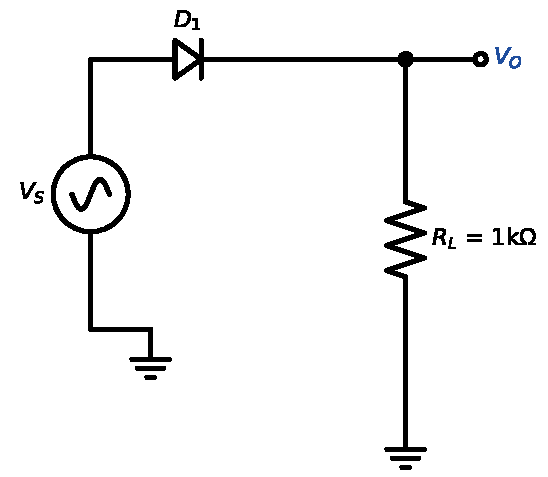
\includegraphics[width=\linewidth,height=5.6cm,keepaspectratio]{p01_circuit}\end{center}
\end{probbox}

\begin{probbox}{Problem 3C.2 \hfill Easy}
The half-wave rectifier below driven by a $60$\,Hz sinusoid of peak $\hat V_S = 12\,\mathrm{V}$ drives $R_L=1\,\mathrm{k}\Omega$ with a filter capacitor $C=100\,\mu \mathrm{F}$. Using the constant-voltage-drop model ($0.7$\,V), find the peak output $V_p$, the ripple $V_r$, the minimum output, the diode currents $I_{D,av}$ and $I_{D,max}$, and the PIV.
\begin{center}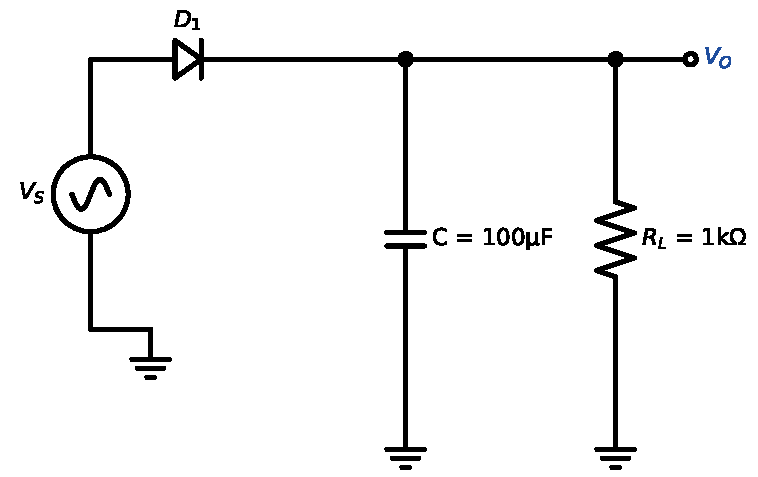
\includegraphics[width=\linewidth,height=5.6cm,keepaspectratio]{p02_circuit}\end{center}
\end{probbox}

\begin{probbox}{Problem 3C.3 \hfill Easy}
The bridge rectifier below driven by a $60$\,Hz sinusoid of peak $\hat V_S = 15\,\mathrm{V}$ drives $R_L=2\,\mathrm{k}\Omega$ (no filter capacitor). Using the constant-voltage-drop model ($0.7$\,V), find the peak output voltage and the peak inverse voltage (PIV) of the diodes, and sketch $V_O(t)$.
\begin{center}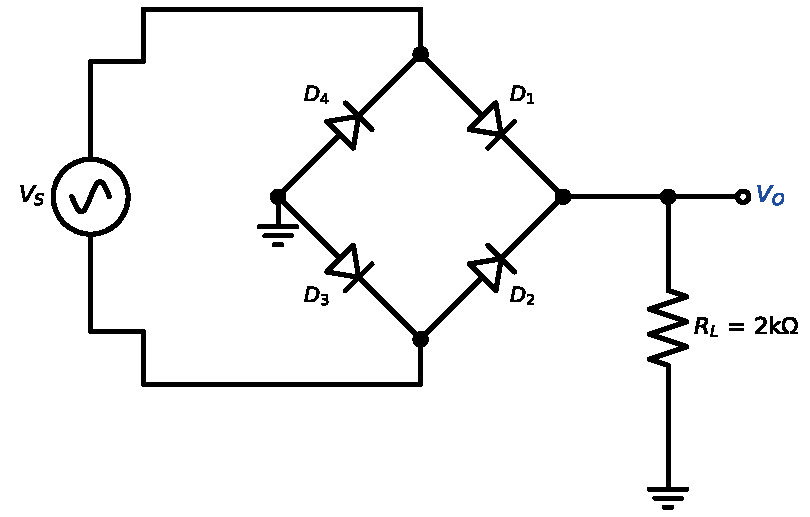
\includegraphics[width=\linewidth,height=5.6cm,keepaspectratio]{p03_circuit}\end{center}
\end{probbox}

\begin{probbox}{Problem 3C.4 \hfill Easy}
The center-tapped full-wave rectifier below driven by a $60$\,Hz sinusoid of peak $\hat V_S = 9\,\mathrm{V}$ on each half of the secondary drives $R_L=1\,\mathrm{k}\Omega$ (no filter capacitor). Using the constant-voltage-drop model ($0.7$\,V), find the peak output voltage and the peak inverse voltage (PIV) of the diodes, and sketch $V_O(t)$.
\begin{center}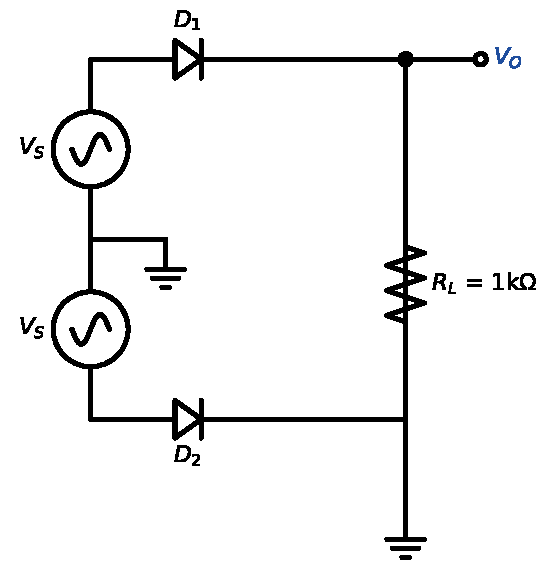
\includegraphics[width=\linewidth,height=5.6cm,keepaspectratio]{p04_circuit}\end{center}
\end{probbox}

\begin{probbox}{Problem 3C.5 \hfill Easy}
The bridge rectifier below driven by a $60$\,Hz sinusoid of peak $\hat V_S = 12\,\mathrm{V}$ drives $R_L=1\,\mathrm{k}\Omega$ with a filter capacitor $C=220\,\mu \mathrm{F}$. Using the constant-voltage-drop model ($0.7$\,V), find the peak output $V_p$, the ripple $V_r$, the minimum output, the diode currents $I_{D,av}$ and $I_{D,max}$, and the PIV.
\begin{center}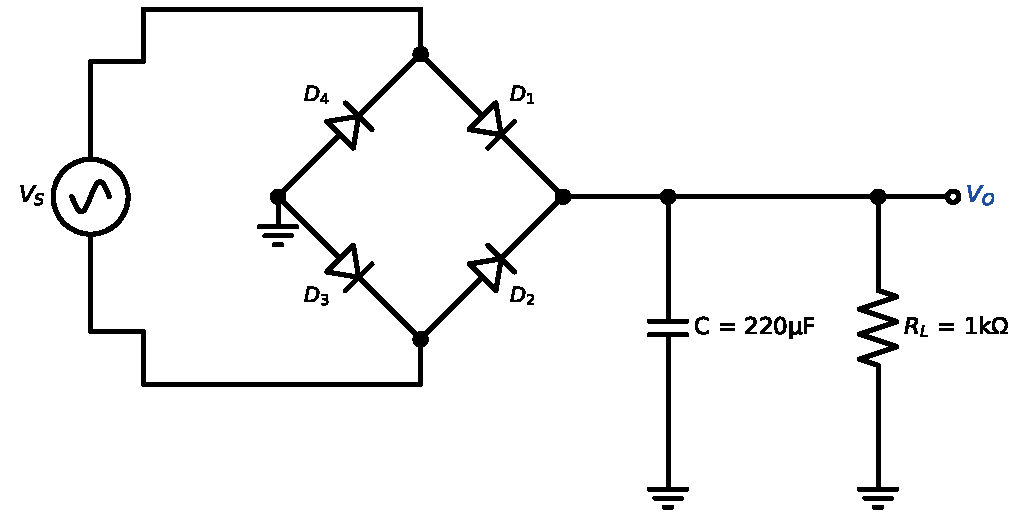
\includegraphics[width=\linewidth,height=5.6cm,keepaspectratio]{p05_circuit}\end{center}
\end{probbox}

\begin{probbox}{Problem 3C.6 \hfill Easy}
The center-tapped full-wave rectifier below driven by a $60$\,Hz sinusoid of peak $\hat V_S = 10\,\mathrm{V}$ on each half of the secondary drives $R_L=500\,\Omega$ with a filter capacitor $C=470\,\mu \mathrm{F}$. Using the constant-voltage-drop model ($0.7$\,V), find the peak output $V_p$, the ripple $V_r$, the minimum output, the diode currents $I_{D,av}$ and $I_{D,max}$, and the PIV.
\begin{center}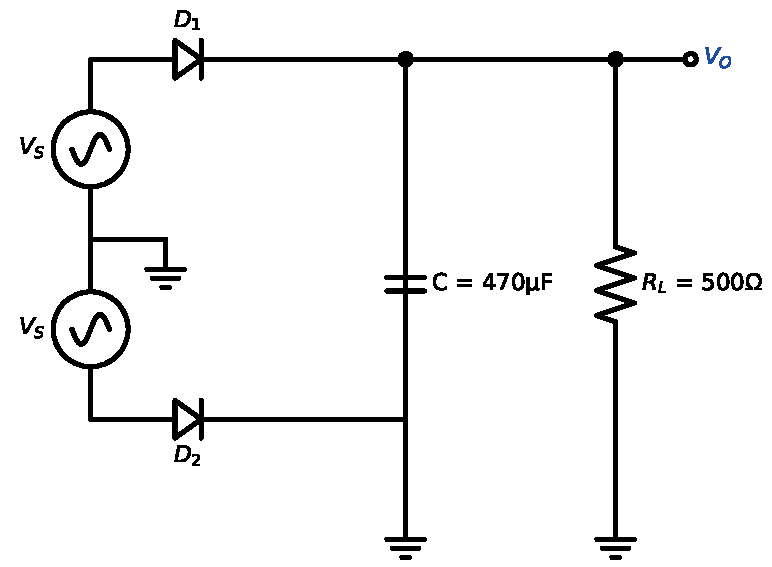
\includegraphics[width=\linewidth,height=5.6cm,keepaspectratio]{p06_circuit}\end{center}
\end{probbox}

\subsection*{Medium problems}
\begin{probbox}{Problem 3C.7 \hfill Medium}
The half-wave rectifier below fed from the $120\,\mathrm{V_{rms}}$, $60$\,Hz mains through a transformer with turns ratio $N=10:1$ drives $R_L=500\,\Omega$ with a filter capacitor $C=470\,\mu \mathrm{F}$. Using the constant-voltage-drop model ($0.7$\,V), find the peak output $V_p$, the ripple $V_r$, the minimum output, the diode currents $I_{D,av}$ and $I_{D,max}$, and the PIV.
\begin{center}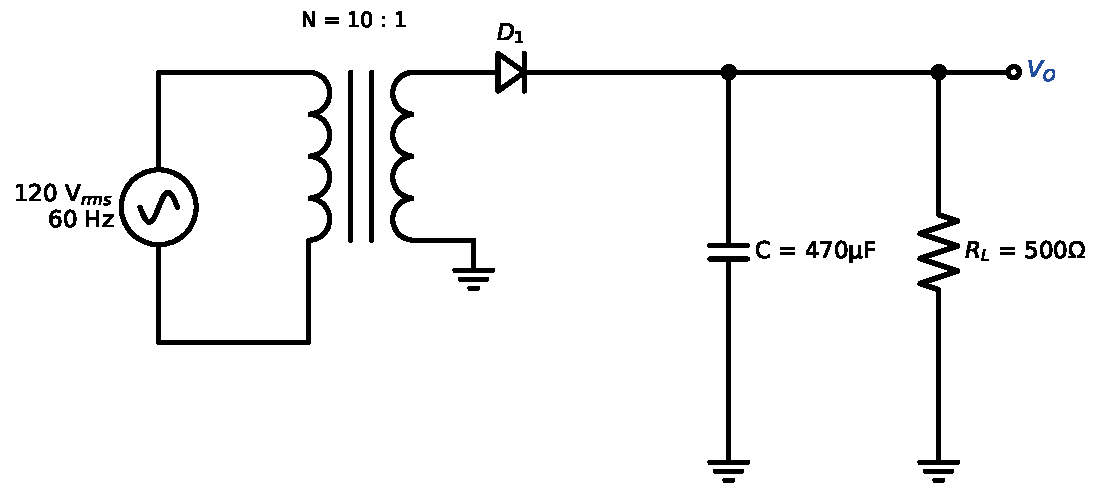
\includegraphics[width=\linewidth,height=5.6cm,keepaspectratio]{p07_circuit}\end{center}
\end{probbox}

\begin{probbox}{Problem 3C.8 \hfill Medium}
The center-tapped full-wave rectifier below fed from the $120\,\mathrm{V_{rms}}$, $60$\,Hz mains through a transformer with turns ratio $N=8:1$ (primary : whole secondary) drives $R_L=200\,\Omega$ with a filter capacitor $C=1\,\mathrm{m}\mathrm{F}$. Using the constant-voltage-drop model ($0.7$\,V), find the peak output $V_p$, the ripple $V_r$, the minimum output, the diode currents $I_{D,av}$ and $I_{D,max}$, and the PIV.
\begin{center}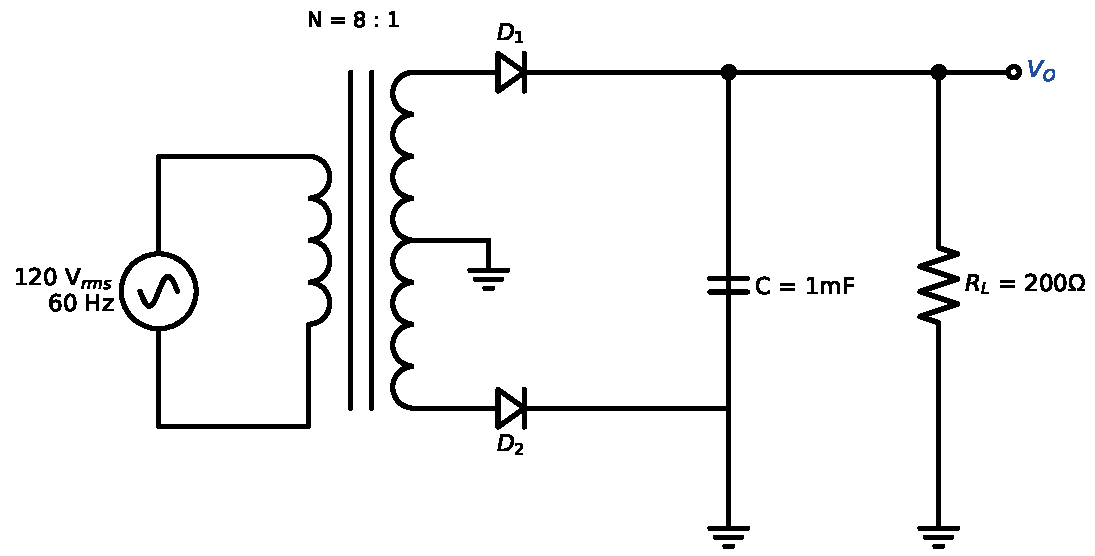
\includegraphics[width=\linewidth,height=5.6cm,keepaspectratio]{p08_circuit}\end{center}
\end{probbox}

\begin{probbox}{Problem 3C.9 \hfill Medium}
The bridge rectifier below fed from the $120\,\mathrm{V_{rms}}$, $60$\,Hz mains through a transformer with turns ratio $N=12:1$ drives $R_L=100\,\Omega$ with a filter capacitor $C=2.2\,\mathrm{m}\mathrm{F}$. Using the constant-voltage-drop model ($0.7$\,V), find the peak output $V_p$, the ripple $V_r$, the minimum output, the diode currents $I_{D,av}$ and $I_{D,max}$, and the PIV.
\begin{center}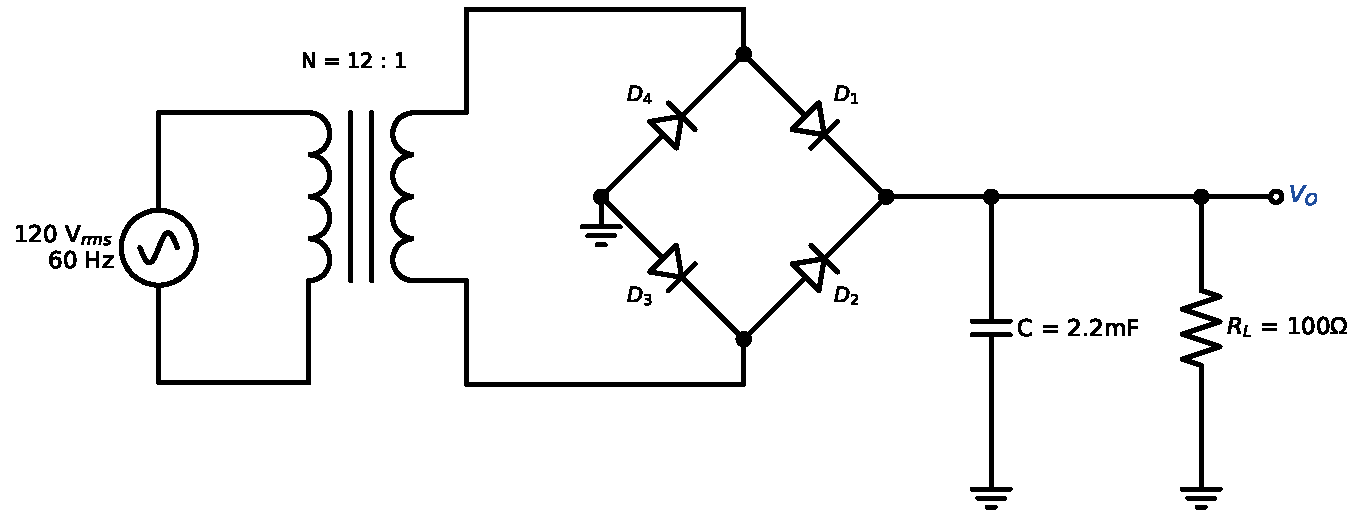
\includegraphics[width=\linewidth,height=5.6cm,keepaspectratio]{p09_circuit}\end{center}
\end{probbox}

\begin{probbox}{Problem 3C.10 \hfill Medium}
The bridge rectifier below driven by a $60$\,Hz sinusoid of peak $\hat V_S = 10\,\mathrm{V}$ drives $R_L=100\,\Omega$. Find the filter capacitance $C$ for a peak-to-peak ripple of at most $500\,\mathrm{m}\mathrm{V}$, the diode currents $I_{D,av}$, $I_{D,max}$ and the peak inverse voltage (PIV) of the diodes. Use the constant-voltage-drop model ($0.7$\,V).
\begin{center}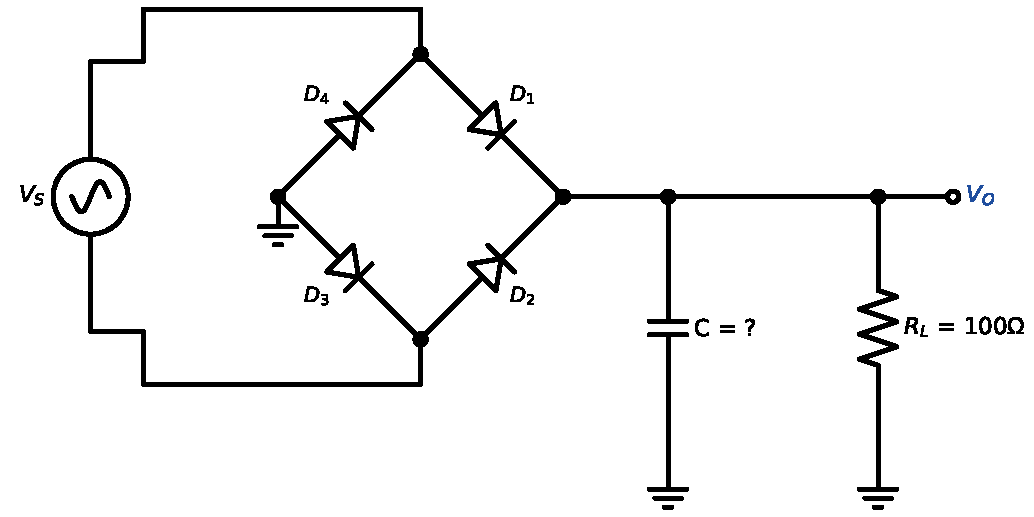
\includegraphics[width=\linewidth,height=5.6cm,keepaspectratio]{p10_circuit}\end{center}
\end{probbox}

\begin{probbox}{Problem 3C.11 \hfill Medium}
The half-wave rectifier below fed from the $120\,\mathrm{V_{rms}}$, $60$\,Hz mains through a transformer with turns ratio $N=12:1$ drives $R_L=1\,\mathrm{k}\Omega$. Find the filter capacitance $C$ for an output that never drops below $11\,\mathrm{V}$, the diode currents $I_{D,av}$, $I_{D,max}$ and the peak inverse voltage (PIV) of the diodes. Use the constant-voltage-drop model ($0.7$\,V).
\begin{center}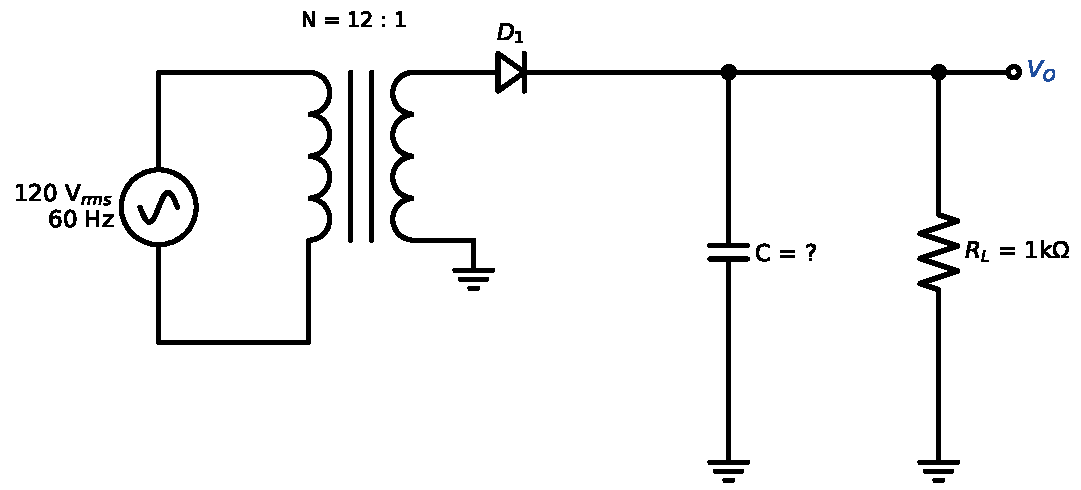
\includegraphics[width=\linewidth,height=5.6cm,keepaspectratio]{p11_circuit}\end{center}
\end{probbox}

\begin{probbox}{Problem 3C.12 \hfill Medium}
The center-tapped full-wave rectifier below fed from the $120\,\mathrm{V_{rms}}$, $60$\,Hz mains through a transformer with turns ratio $N=10:1$ (primary : whole secondary) drives $R_L=50\,\Omega$. Find the filter capacitance $C$ for a peak-to-peak ripple of at most $400\,\mathrm{m}\mathrm{V}$, the diode currents $I_{D,av}$, $I_{D,max}$ and the peak inverse voltage (PIV) of the diodes. Use the constant-voltage-drop model ($0.7$\,V).
\begin{center}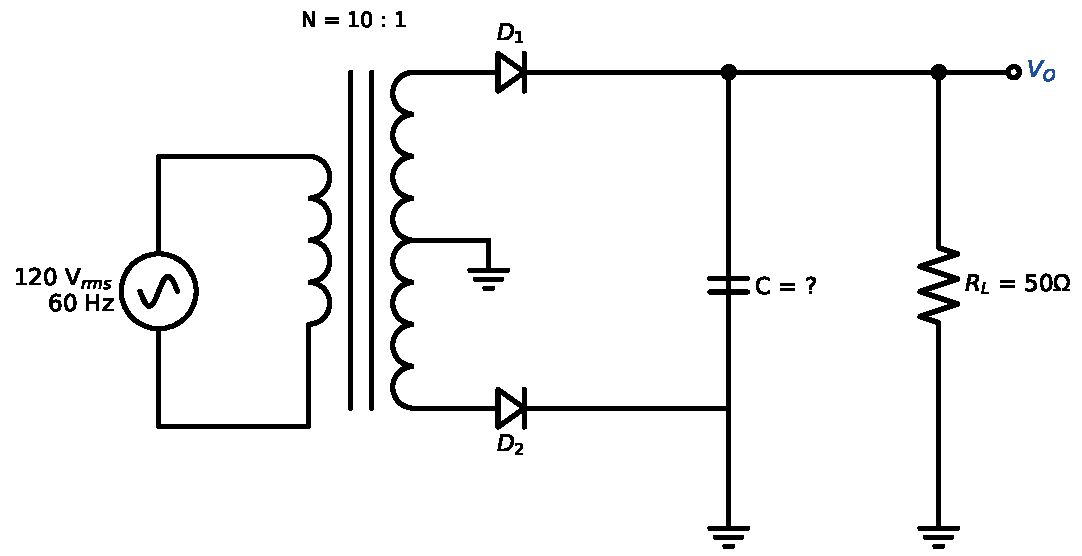
\includegraphics[width=\linewidth,height=5.6cm,keepaspectratio]{p12_circuit}\end{center}
\end{probbox}

\subsection*{Hard problems}
\begin{probbox}{Problem 3C.13 \hfill Hard}
Design an AC adapter using a single transformer and a bridge rectifier (constant-voltage-drop diodes, $0.7$\,V; mains $120\,\mathrm{V_{rms}}$, $60$\,Hz) for: output voltage $V_o=3\,\mathrm{V}$, maximum ripple $5\%$, load current $0$--$400\,\mathrm{m}\mathrm{A}$. Find the transformer ratio $N$, the capacitance $C$ and the minimum diode ratings ($I_{D,max}$, $I_{D,av}$, reverse breakdown voltage).
\begin{center}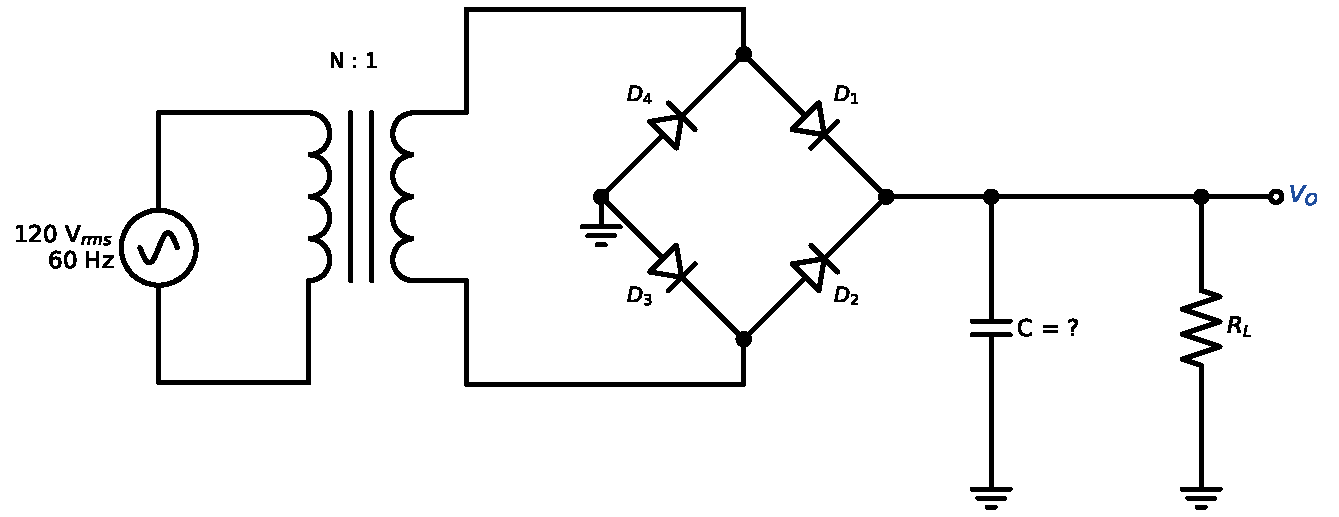
\includegraphics[width=\linewidth,height=5.6cm,keepaspectratio]{p13_circuit}\end{center}
\end{probbox}

\begin{probbox}{Problem 3C.14 \hfill Hard}
Design an AC adapter using a center-tapped transformer and a full-wave rectifier (constant-voltage-drop diodes, $0.7$\,V; mains $120\,\mathrm{V_{rms}}$, $60$\,Hz) for: output voltage $V_o=5\,\mathrm{V}$, maximum ripple $10\%$, load current $0$--$1.5\,\mathrm{A}$. Find the transformer ratio $N$, the capacitance $C$ and the minimum diode ratings ($I_{D,max}$, $I_{D,av}$, reverse breakdown voltage).
\begin{center}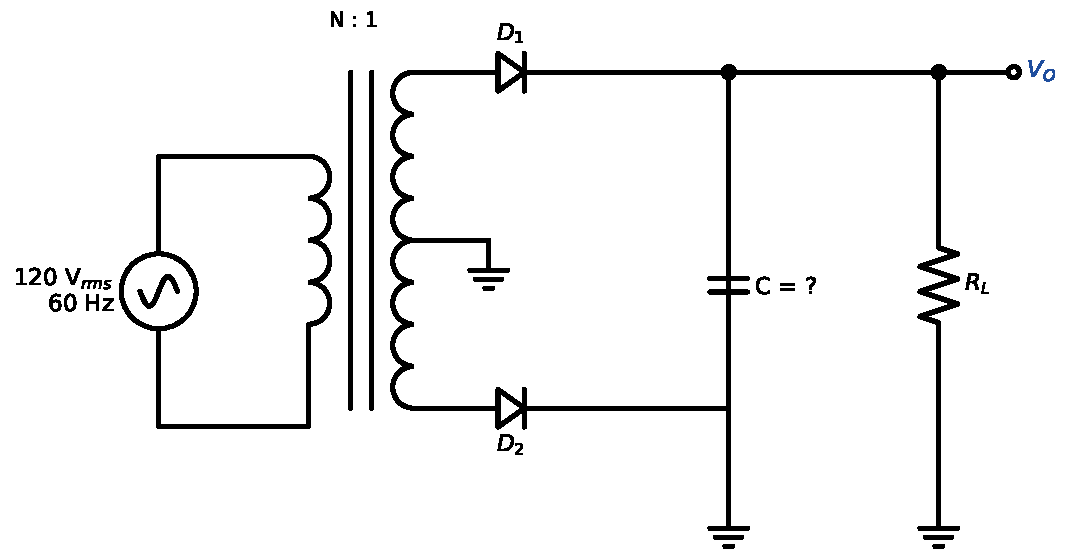
\includegraphics[width=\linewidth,height=5.6cm,keepaspectratio]{p14_circuit}\end{center}
\end{probbox}

\begin{probbox}{Problem 3C.15 \hfill Hard}
Design an AC adapter using a single transformer and a bridge rectifier (constant-voltage-drop diodes, $0.7$\,V; mains $120\,\mathrm{V_{rms}}$, $60$\,Hz) for: output voltage $V_o=12\,\mathrm{V}$, maximum ripple $5\%$, load current $0$--$1\,\mathrm{A}$. Find the transformer ratio $N$, the capacitance $C$ and the minimum diode ratings ($I_{D,max}$, $I_{D,av}$, reverse breakdown voltage).
\begin{center}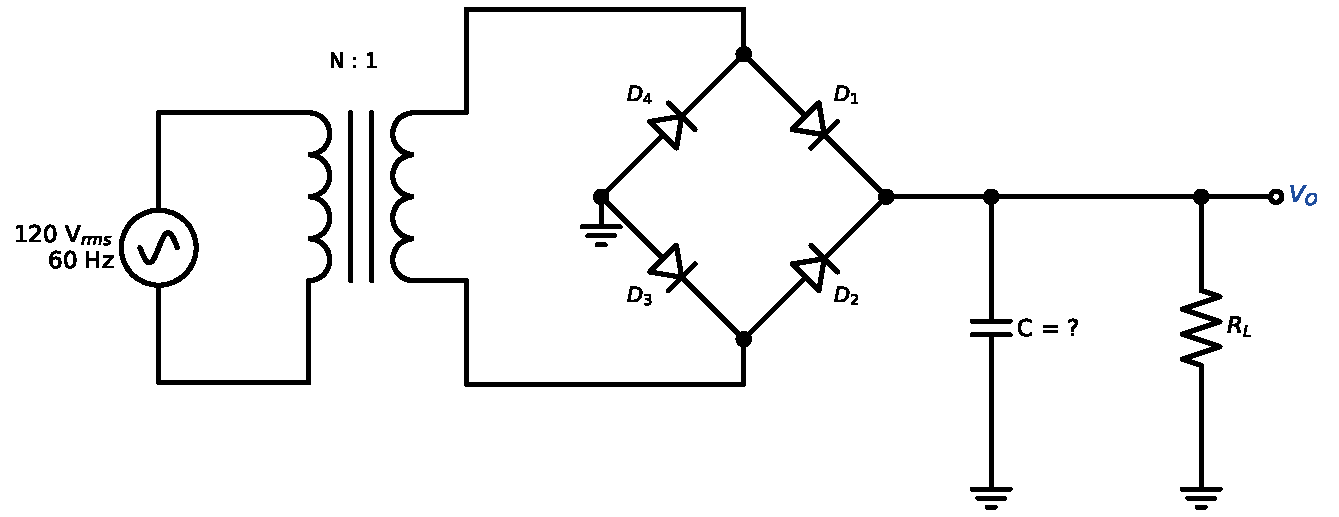
\includegraphics[width=\linewidth,height=5.6cm,keepaspectratio]{p15_circuit}\end{center}
\end{probbox}

\begin{probbox}{Problem 3C.16 \hfill Hard}
Design an AC adapter using a center-tapped transformer and a full-wave rectifier (constant-voltage-drop diodes, $0.7$\,V; mains $120\,\mathrm{V_{rms}}$, $60$\,Hz) for: output voltage $V_o=9\,\mathrm{V}$, maximum ripple $5\%$, load current $0$--$500\,\mathrm{m}\mathrm{A}$. Find the transformer ratio $N$, the capacitance $C$ and the minimum diode ratings ($I_{D,max}$, $I_{D,av}$, reverse breakdown voltage).
\begin{center}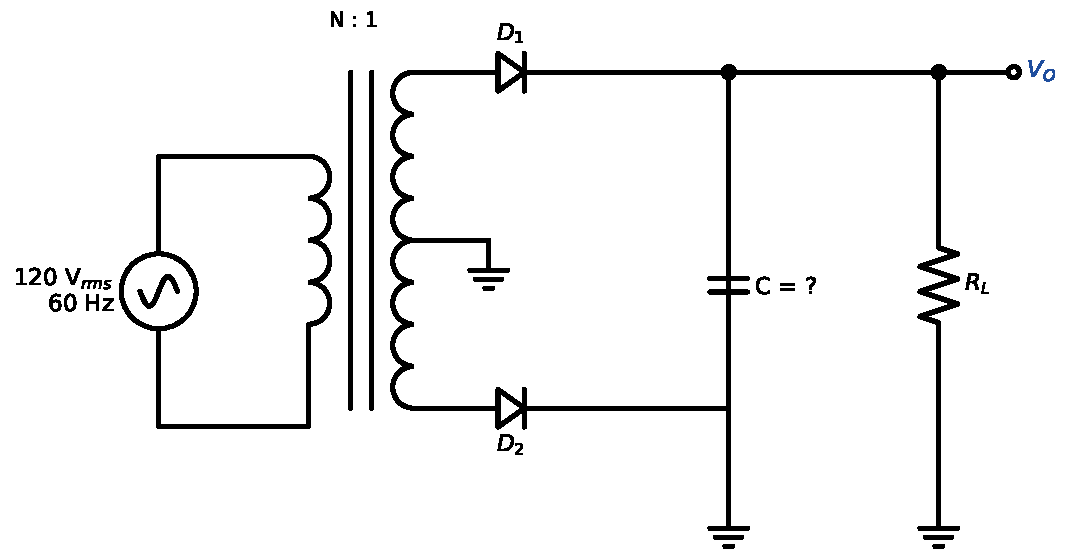
\includegraphics[width=\linewidth,height=5.6cm,keepaspectratio]{p16_circuit}\end{center}
\end{probbox}

\begin{probbox}{Problem 3C.17 \hfill Hard}
Design an AC adapter using a transformer and a half-wave rectifier (constant-voltage-drop diodes, $0.7$\,V; mains $120\,\mathrm{V_{rms}}$, $60$\,Hz) for: output voltage $V_o=5\,\mathrm{V}$, maximum ripple $10\%$, load current $0$--$100\,\mathrm{m}\mathrm{A}$. Find the transformer ratio $N$, the capacitance $C$ and the minimum diode ratings ($I_{D,max}$, $I_{D,av}$, reverse breakdown voltage).
\begin{center}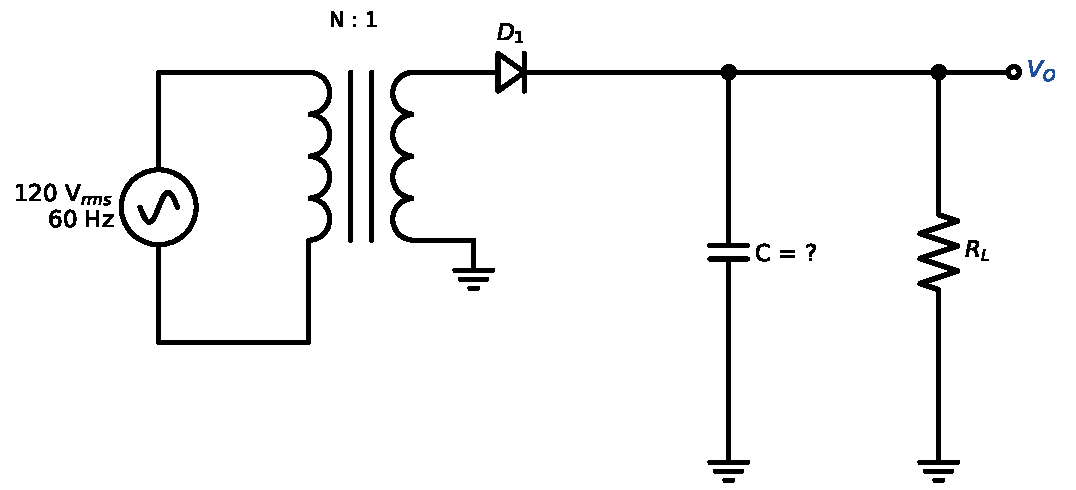
\includegraphics[width=\linewidth,height=5.6cm,keepaspectratio]{p17_circuit}\end{center}
\end{probbox}

\begin{probbox}{Problem 3C.18 \hfill Hard}
Design an AC adapter using a single transformer and a bridge rectifier (constant-voltage-drop diodes, $0.7$\,V; mains $120\,\mathrm{V_{rms}}$, $60$\,Hz) for: output voltage $V_o=15\,\mathrm{V}$, maximum ripple $5\%$, load current $0$--$800\,\mathrm{m}\mathrm{A}$. Find the transformer ratio $N$, the capacitance $C$ and the minimum diode ratings ($I_{D,max}$, $I_{D,av}$, reverse breakdown voltage).
\begin{center}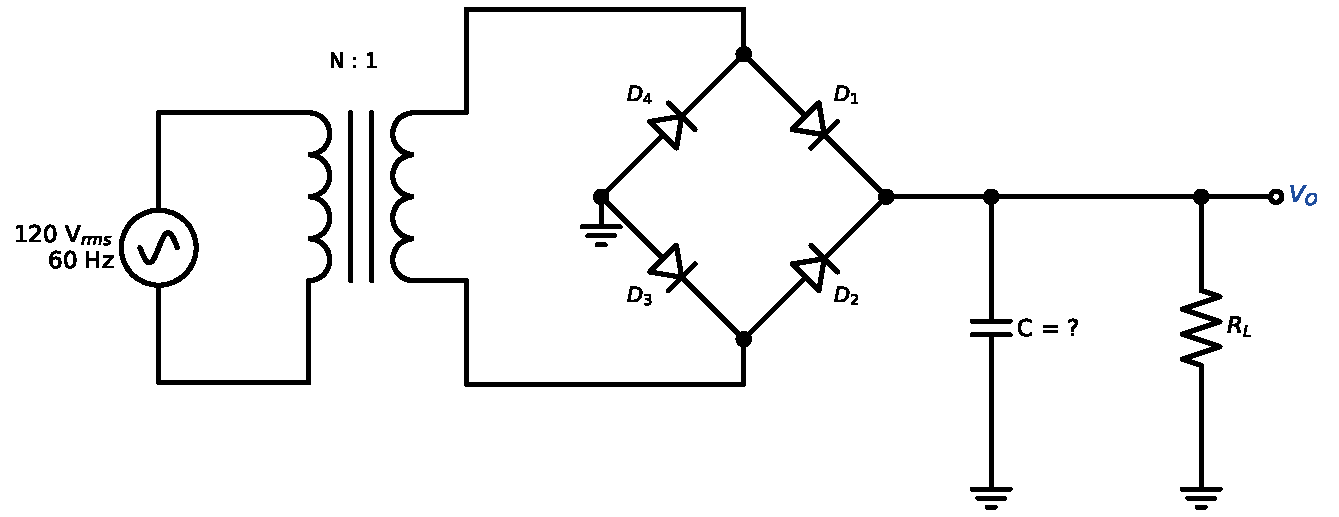
\includegraphics[width=\linewidth,height=5.6cm,keepaspectratio]{p18_circuit}\end{center}
\end{probbox}

\newpage
\section*{Solutions}
Every solution follows the steps of the Lecture-3 pipeline card.
\newpage
\subsection*{Solution 3C.1 \hfill Easy}
\begin{center}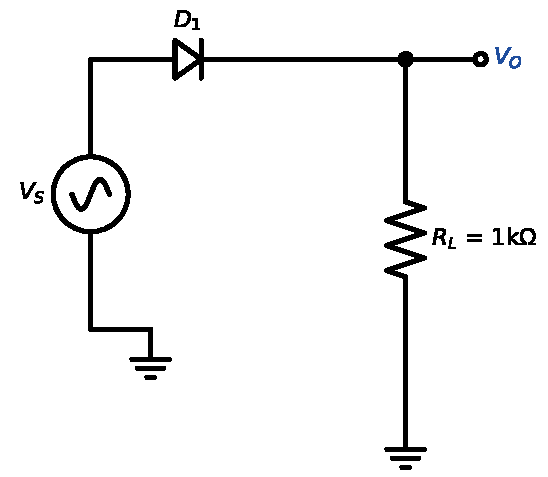
\includegraphics[width=0.9\linewidth,height=5cm,keepaspectratio]{p01_circuit}\end{center}
\solstep{1}{Peak output}At the peak of the input the current flows through the single diode, each dropping $0.7$\,V (tool T1):\[
V_p = \hat V_S - 0.7 = 10 - 0.7 = 9.3\,\mathrm{V},\qquad I_L \approx \frac{V_p}{R_L} = 9.3\,\mathrm{m}\mathrm{A}
\]

\solstep{2}{Peak inverse voltage}At the negative peak the diode is OFF, the output is 0 and the whole $\hat V_S$ appears across the diode: PIV $= \hat V_S = 10\,\mathrm{V}$. The diodes must have a reverse breakdown voltage above the PIV.
\solstep{3}{Waveforms}\begin{center}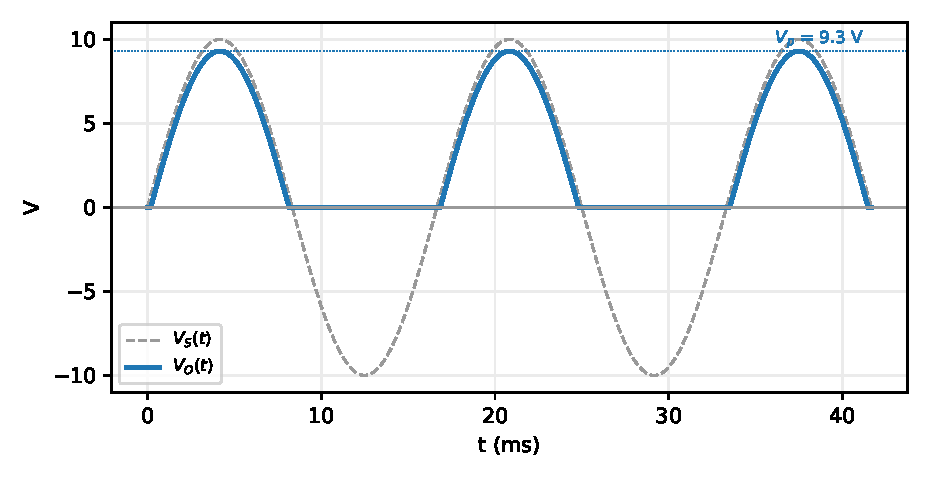
\includegraphics[width=0.7\linewidth,height=5.5cm,keepaspectratio]{p01_wave}\end{center}

\begin{ansbox}
$V_p = 9.3\,\mathrm{V}$,\quad PIV $= 10\,\mathrm{V}$
\end{ansbox}

\newpage
\subsection*{Solution 3C.2 \hfill Easy}
\begin{center}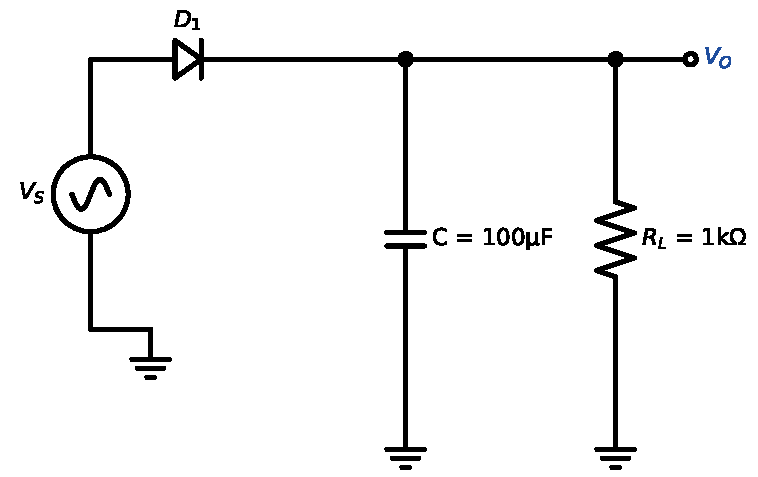
\includegraphics[width=0.9\linewidth,height=5cm,keepaspectratio]{p02_circuit}\end{center}
\solstep{1}{Peak output}At the peak of the input the current flows through the single diode, each dropping $0.7$\,V (tool T1):\[
V_p = \hat V_S - 0.7 = 12 - 0.7 = 11.3\,\mathrm{V},\qquad I_L \approx \frac{V_p}{R_L} = 11.3\,\mathrm{m}\mathrm{A}
\]

\solstep{2}{Ripple}Half-wave: the capacitor is recharged once per period, $T = 1/60$\,s. Between recharges the capacitor discharges through $R_L$ (tool T4):\[
V_r \approx V_p\frac{T}{R_LC} = \frac{11.3\times 0.01667}{1000\times 10^{-4}} = 1.88\,\mathrm{V}
\]
so the output swings between $V_p = 11.3\,\mathrm{V}$ and $V_p - V_r = 9.42\,\mathrm{V}$ (average $\approx V_p - V_r/2 = 10.4\,\mathrm{V}$).
\solstep{3}{Diode currents}The diodes only conduct during the short recharge interval, so they must deliver a whole period's charge in a short burst (tool T4):\begin{align*}
\sqrt{2V_p/V_r} &= \sqrt{2\times11.3/1.883} = 3.464 \\
I_{D,av} &= I_L\left(1+\pi\sqrt{2V_p/V_r}\right) = 0.0113\left(1+\pi\times3.464\right) = 134\,\mathrm{m}\mathrm{A} \\
I_{D,max} &= I_L\left(1+2\pi\sqrt{2V_p/V_r}\right) = 257\,\mathrm{m}\mathrm{A}
\end{align*}

\solstep{4}{Peak inverse voltage}At the negative peak the anode is at $-\hat V_S$ while the capacitor holds the cathode near $V_p$: PIV $= \hat V_S + V_p = 2\hat V_S - 0.7 = 23.3\,\mathrm{V}$. The diodes must have a reverse breakdown voltage above the PIV.
\solstep{5}{Waveforms}\begin{center}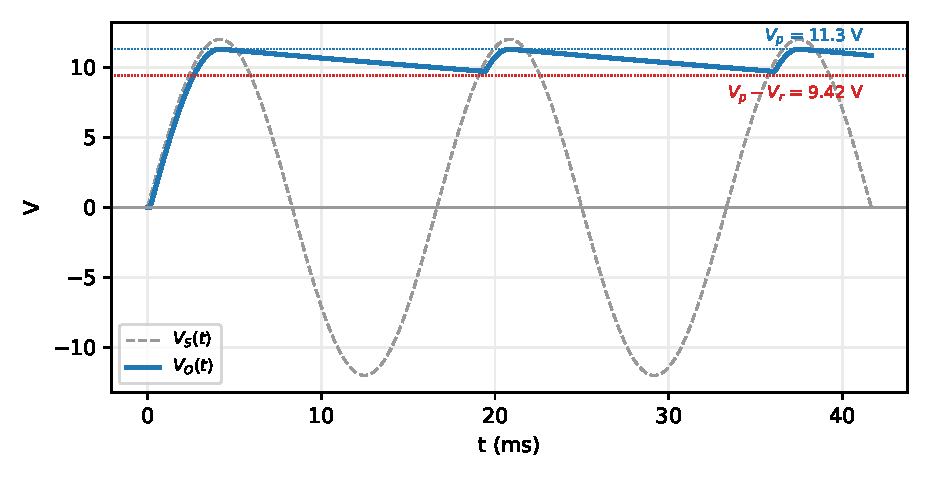
\includegraphics[width=0.7\linewidth,height=5.5cm,keepaspectratio]{p02_wave}\end{center}
 The ripple formula assumes the capacitor discharges for a whole $T$; in reality it is recharged a little earlier, so the true ripple (plotted) is slightly smaller --- the formula errs on the safe side.
\begin{ansbox}
$V_p = 11.3\,\mathrm{V}$,\quad $V_r = 1.88\,\mathrm{V}$,\quad $V_{o,min} = 9.42\,\mathrm{V}$,\quad $I_{D,av} = 134\,\mathrm{m}\mathrm{A}$,\quad $I_{D,max} = 257\,\mathrm{m}\mathrm{A}$,\quad PIV $= 23.3\,\mathrm{V}$
\end{ansbox}

\newpage
\subsection*{Solution 3C.3 \hfill Easy}
\begin{center}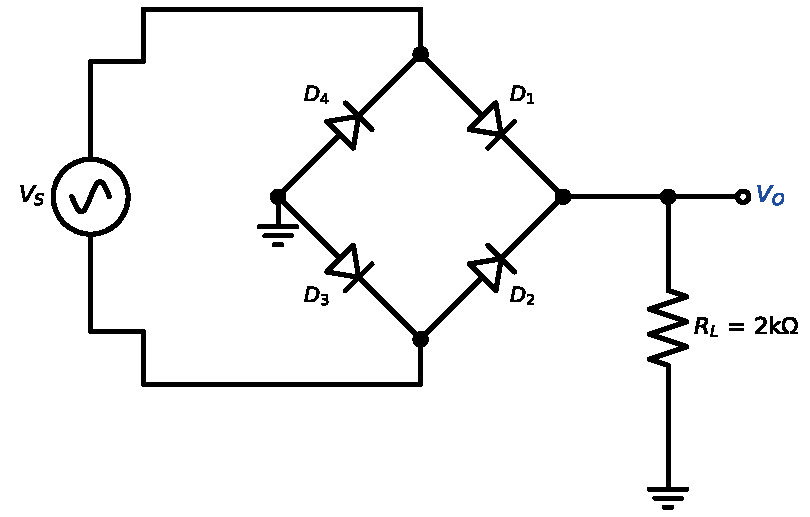
\includegraphics[width=0.9\linewidth,height=5cm,keepaspectratio]{p03_circuit}\end{center}
\solstep{1}{Peak output}At the peak of the input the current flows through two diodes in series (one on each side of the bridge), each dropping $0.7$\,V (tool T1):\[
V_p = \hat V_S - 1.4 = 15 - 1.4 = 13.6\,\mathrm{V},\qquad I_L \approx \frac{V_p}{R_L} = 6.8\,\mathrm{m}\mathrm{A}
\]

\solstep{2}{Peak inverse voltage}When a pair of diodes conducts, each of the other two sees the output plus one diode drop: PIV $= V_p + 0.7 = \hat V_S - 0.7 = 14.3\,\mathrm{V}$. The diodes must have a reverse breakdown voltage above the PIV.
\solstep{3}{Waveforms}\begin{center}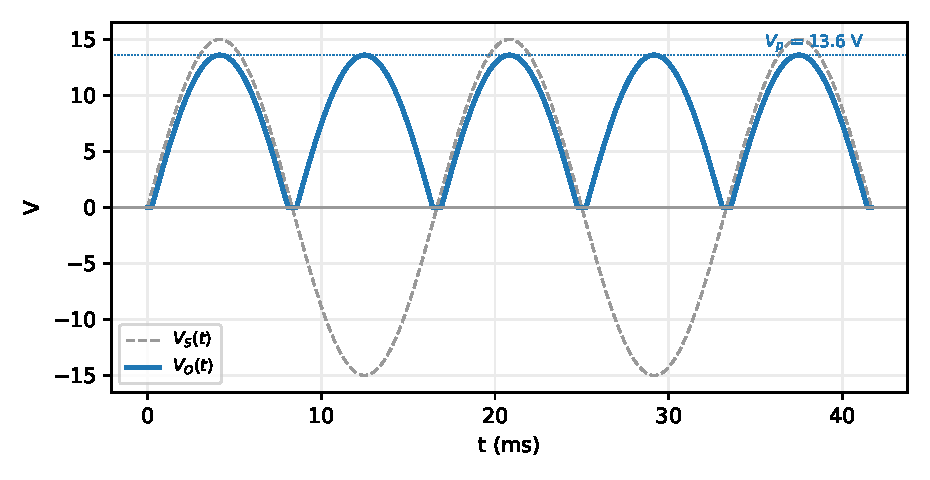
\includegraphics[width=0.7\linewidth,height=5.5cm,keepaspectratio]{p03_wave}\end{center}

\begin{ansbox}
$V_p = 13.6\,\mathrm{V}$,\quad PIV $= 14.3\,\mathrm{V}$
\end{ansbox}

\newpage
\subsection*{Solution 3C.4 \hfill Easy}
\begin{center}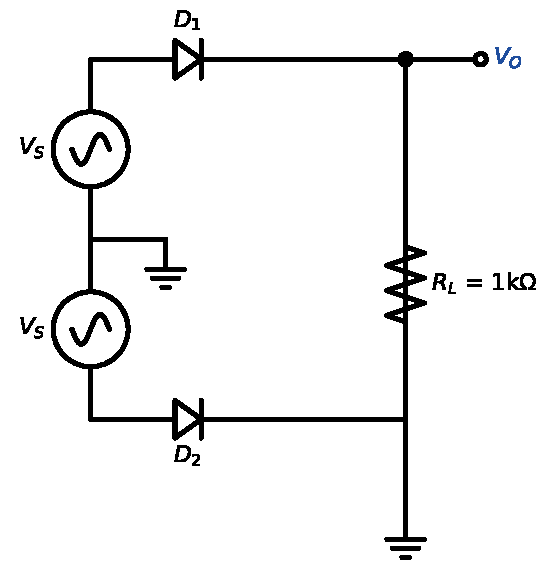
\includegraphics[width=0.9\linewidth,height=5cm,keepaspectratio]{p04_circuit}\end{center}
\solstep{1}{Peak output}At the peak of the input the current flows through one diode (each half of the secondary has its own diode), each dropping $0.7$\,V (tool T1):\[
V_p = \hat V_S - 0.7 = 9 - 0.7 = 8.3\,\mathrm{V},\qquad I_L \approx \frac{V_p}{R_L} = 8.3\,\mathrm{m}\mathrm{A}
\]

\solstep{2}{Peak inverse voltage}When one diode conducts its cathode sits at $V_p = \hat V_S - 0.7$ while its own half of the secondary is at $-\hat V_S$: PIV $= 2\hat V_S - 0.7 = 17.3\,\mathrm{V}$. The diodes must have a reverse breakdown voltage above the PIV.
\solstep{3}{Waveforms}\begin{center}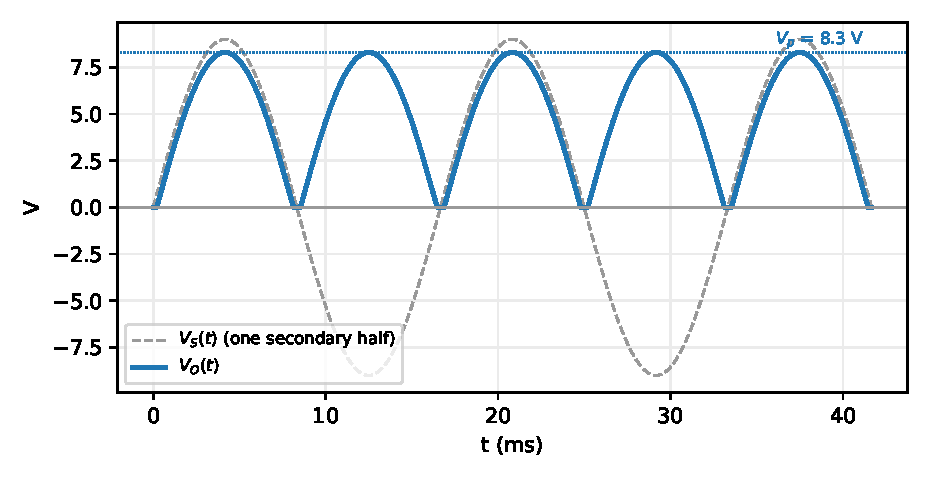
\includegraphics[width=0.7\linewidth,height=5.5cm,keepaspectratio]{p04_wave}\end{center}

\begin{ansbox}
$V_p = 8.3\,\mathrm{V}$,\quad PIV $= 17.3\,\mathrm{V}$
\end{ansbox}

\newpage
\subsection*{Solution 3C.5 \hfill Easy}
\begin{center}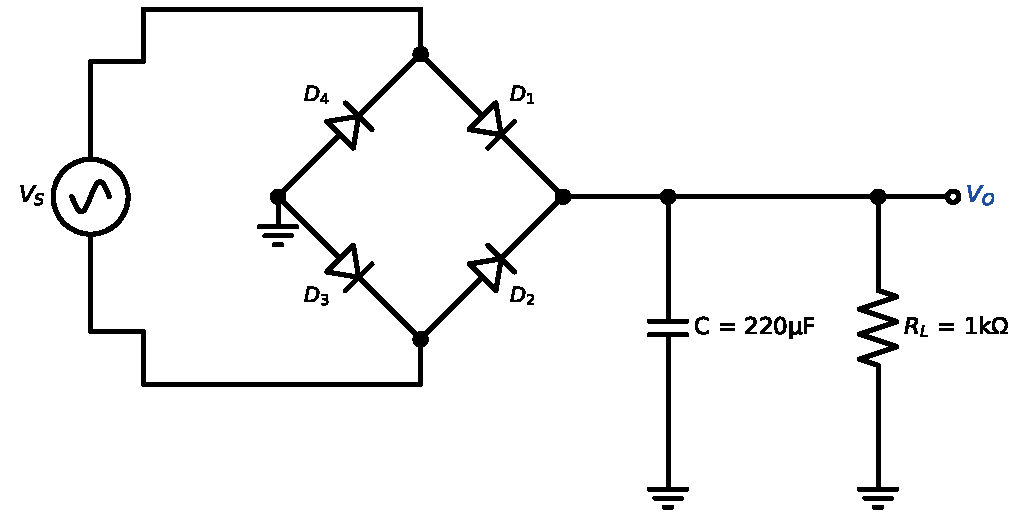
\includegraphics[width=0.9\linewidth,height=5cm,keepaspectratio]{p05_circuit}\end{center}
\solstep{1}{Peak output}At the peak of the input the current flows through two diodes in series (one on each side of the bridge), each dropping $0.7$\,V (tool T1):\[
V_p = \hat V_S - 1.4 = 12 - 1.4 = 10.6\,\mathrm{V},\qquad I_L \approx \frac{V_p}{R_L} = 10.6\,\mathrm{m}\mathrm{A}
\]

\solstep{2}{Ripple}Full-wave: the capacitor is recharged every half period, $T = 1/120$\,s. Between recharges the capacitor discharges through $R_L$ (tool T4):\[
V_r \approx V_p\frac{T}{R_LC} = \frac{10.6\times 0.008333}{1000\times 2.2\times 10^{-4}} = 402\,\mathrm{m}\mathrm{V}
\]
so the output swings between $V_p = 10.6\,\mathrm{V}$ and $V_p - V_r = 10.2\,\mathrm{V}$ (average $\approx V_p - V_r/2 = 10.4\,\mathrm{V}$).
\solstep{3}{Diode currents}The diodes only conduct during the short recharge interval, so they must deliver a whole period's charge in a short burst (tool T4):\begin{align*}
\sqrt{2V_p/V_r} &= \sqrt{2\times10.6/0.4015} = 7.266 \\
I_{D,av} &= I_L\left(1+\pi\sqrt{2V_p/V_r}\right) = 0.0106\left(1+\pi\times7.266\right) = 253\,\mathrm{m}\mathrm{A} \\
I_{D,max} &= I_L\left(1+2\pi\sqrt{2V_p/V_r}\right) = 495\,\mathrm{m}\mathrm{A}
\end{align*}

\solstep{4}{Peak inverse voltage}When a pair of diodes conducts, each of the other two sees the output plus one diode drop: PIV $= V_p + 0.7 = \hat V_S - 0.7 = 11.3\,\mathrm{V}$. The diodes must have a reverse breakdown voltage above the PIV.
\solstep{5}{Waveforms}\begin{center}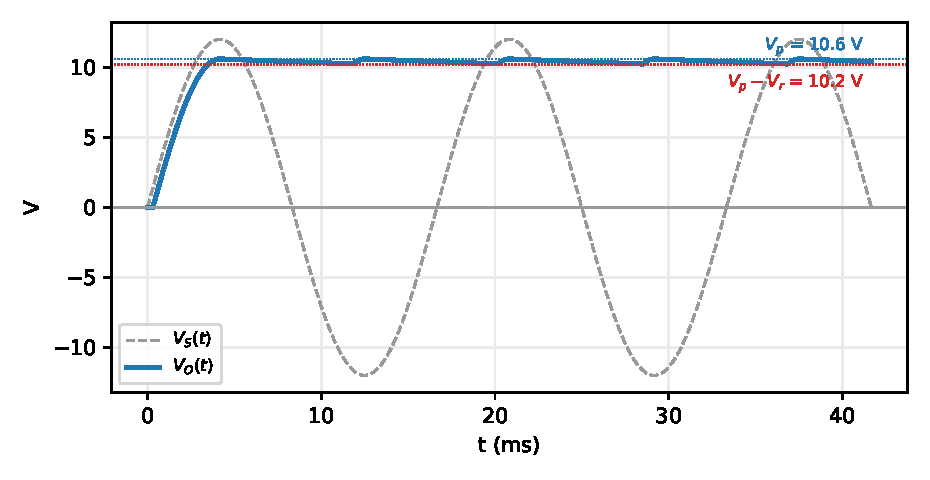
\includegraphics[width=0.7\linewidth,height=5.5cm,keepaspectratio]{p05_wave}\end{center}
 The ripple formula assumes the capacitor discharges for a whole $T$; in reality it is recharged a little earlier, so the true ripple (plotted) is slightly smaller --- the formula errs on the safe side.
\begin{ansbox}
$V_p = 10.6\,\mathrm{V}$,\quad $V_r = 402\,\mathrm{m}\mathrm{V}$,\quad $V_{o,min} = 10.2\,\mathrm{V}$,\quad $I_{D,av} = 253\,\mathrm{m}\mathrm{A}$,\quad $I_{D,max} = 495\,\mathrm{m}\mathrm{A}$,\quad PIV $= 11.3\,\mathrm{V}$
\end{ansbox}

\newpage
\subsection*{Solution 3C.6 \hfill Easy}
\begin{center}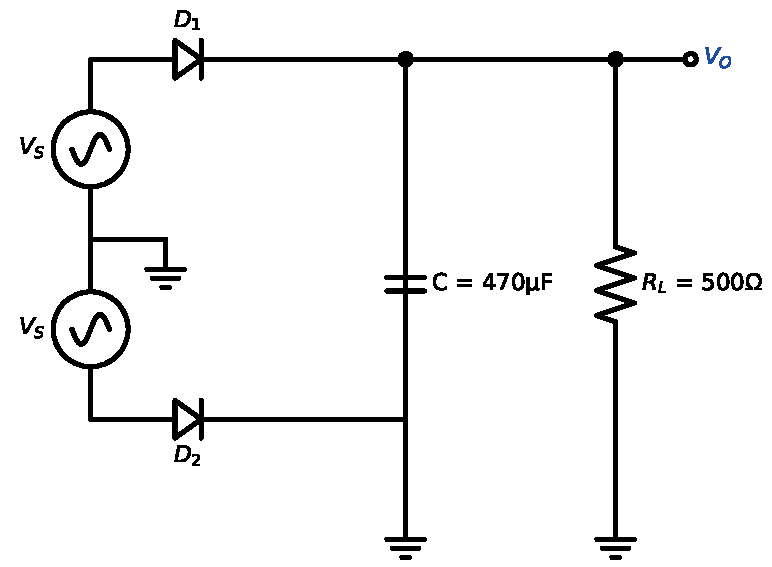
\includegraphics[width=0.9\linewidth,height=5cm,keepaspectratio]{p06_circuit}\end{center}
\solstep{1}{Peak output}At the peak of the input the current flows through one diode (each half of the secondary has its own diode), each dropping $0.7$\,V (tool T1):\[
V_p = \hat V_S - 0.7 = 10 - 0.7 = 9.3\,\mathrm{V},\qquad I_L \approx \frac{V_p}{R_L} = 18.6\,\mathrm{m}\mathrm{A}
\]

\solstep{2}{Ripple}Full-wave: the capacitor is recharged every half period, $T = 1/120$\,s. Between recharges the capacitor discharges through $R_L$ (tool T4):\[
V_r \approx V_p\frac{T}{R_LC} = \frac{9.3\times 0.008333}{500\times 4.7\times 10^{-4}} = 330\,\mathrm{m}\mathrm{V}
\]
so the output swings between $V_p = 9.3\,\mathrm{V}$ and $V_p - V_r = 8.97\,\mathrm{V}$ (average $\approx V_p - V_r/2 = 9.14\,\mathrm{V}$).
\solstep{3}{Diode currents}The diodes only conduct during the short recharge interval, so they must deliver a whole period's charge in a short burst (tool T4):\begin{align*}
\sqrt{2V_p/V_r} &= \sqrt{2\times9.3/0.3298} = 7.51 \\
I_{D,av} &= I_L\left(1+\pi\sqrt{2V_p/V_r}\right) = 0.0186\left(1+\pi\times7.51\right) = 457\,\mathrm{m}\mathrm{A} \\
I_{D,max} &= I_L\left(1+2\pi\sqrt{2V_p/V_r}\right) = 896\,\mathrm{m}\mathrm{A}
\end{align*}

\solstep{4}{Peak inverse voltage}When one diode conducts its cathode sits at $V_p = \hat V_S - 0.7$ while its own half of the secondary is at $-\hat V_S$: PIV $= 2\hat V_S - 0.7 = 19.3\,\mathrm{V}$. The diodes must have a reverse breakdown voltage above the PIV.
\solstep{5}{Waveforms}\begin{center}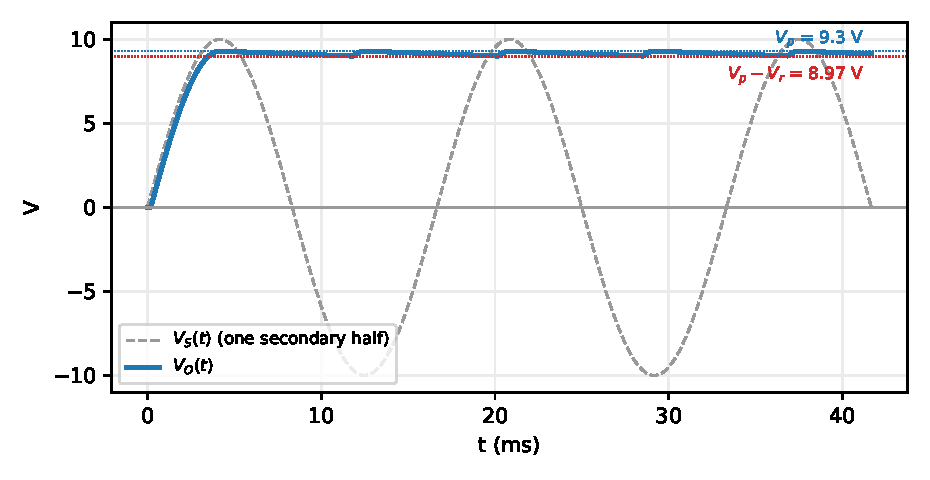
\includegraphics[width=0.7\linewidth,height=5.5cm,keepaspectratio]{p06_wave}\end{center}
 The ripple formula assumes the capacitor discharges for a whole $T$; in reality it is recharged a little earlier, so the true ripple (plotted) is slightly smaller --- the formula errs on the safe side.
\begin{ansbox}
$V_p = 9.3\,\mathrm{V}$,\quad $V_r = 330\,\mathrm{m}\mathrm{V}$,\quad $V_{o,min} = 8.97\,\mathrm{V}$,\quad $I_{D,av} = 457\,\mathrm{m}\mathrm{A}$,\quad $I_{D,max} = 896\,\mathrm{m}\mathrm{A}$,\quad PIV $= 19.3\,\mathrm{V}$
\end{ansbox}

\newpage
\subsection*{Solution 3C.7 \hfill Medium}
\begin{center}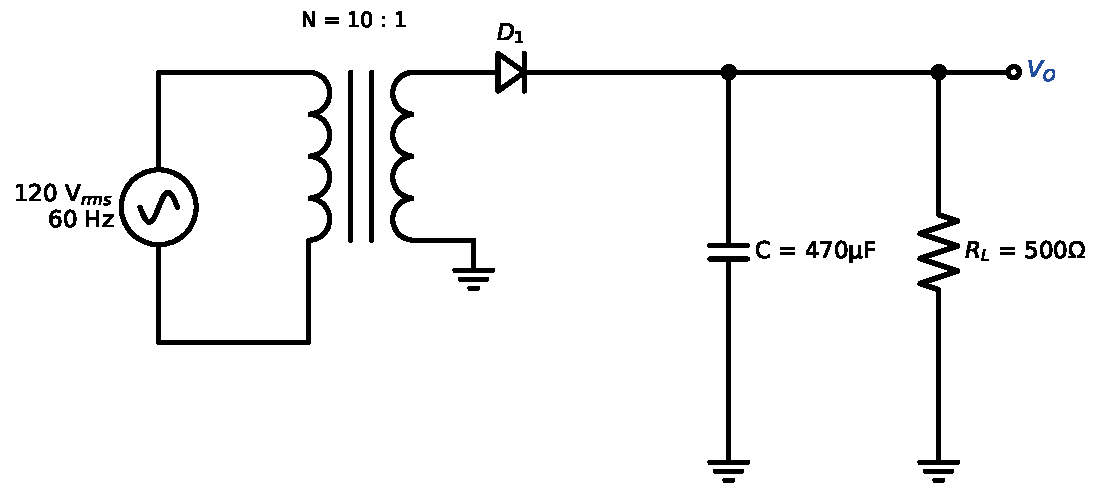
\includegraphics[width=0.9\linewidth,height=5cm,keepaspectratio]{p07_circuit}\end{center}
\solstep{1}{Secondary voltage}The mains peak is $120\sqrt2 = 170$\,V, so the secondary peaks at $\frac{170}{N} = 17\,\mathrm{V}$ $=\hat V_S$.
\solstep{2}{Peak output}At the peak of the input the current flows through the single diode, each dropping $0.7$\,V (tool T1):\[
V_p = \hat V_S - 0.7 = 17 - 0.7 = 16.3\,\mathrm{V},\qquad I_L \approx \frac{V_p}{R_L} = 32.6\,\mathrm{m}\mathrm{A}
\]

\solstep{3}{Ripple}Half-wave: the capacitor is recharged once per period, $T = 1/60$\,s. Between recharges the capacitor discharges through $R_L$ (tool T4):\[
V_r \approx V_p\frac{T}{R_LC} = \frac{16.3\times 0.01667}{500\times 4.7\times 10^{-4}} = 1.16\,\mathrm{V}
\]
so the output swings between $V_p = 16.3\,\mathrm{V}$ and $V_p - V_r = 15.1\,\mathrm{V}$ (average $\approx V_p - V_r/2 = 15.7\,\mathrm{V}$).
\solstep{4}{Diode currents}The diodes only conduct during the short recharge interval, so they must deliver a whole period's charge in a short burst (tool T4):\begin{align*}
\sqrt{2V_p/V_r} &= \sqrt{2\times16.3/1.156} = 5.31 \\
I_{D,av} &= I_L\left(1+\pi\sqrt{2V_p/V_r}\right) = 0.0326\left(1+\pi\times5.31\right) = 576\,\mathrm{m}\mathrm{A} \\
I_{D,max} &= I_L\left(1+2\pi\sqrt{2V_p/V_r}\right) = 1.12\,\mathrm{A}
\end{align*}

\solstep{5}{Peak inverse voltage}At the negative peak the anode is at $-\hat V_S$ while the capacitor holds the cathode near $V_p$: PIV $= \hat V_S + V_p = 2\hat V_S - 0.7 = 33.3\,\mathrm{V}$. The diodes must have a reverse breakdown voltage above the PIV.
\solstep{6}{Waveforms}\begin{center}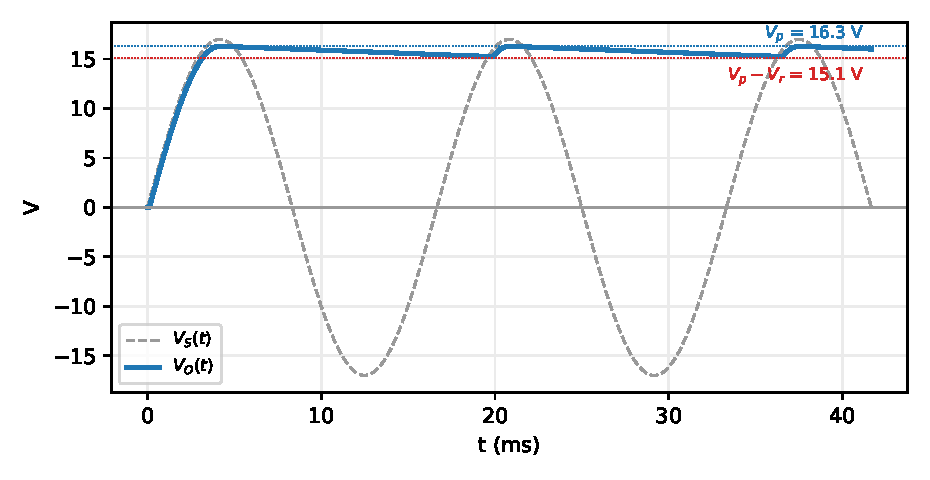
\includegraphics[width=0.7\linewidth,height=5.5cm,keepaspectratio]{p07_wave}\end{center}
 The ripple formula assumes the capacitor discharges for a whole $T$; in reality it is recharged a little earlier, so the true ripple (plotted) is slightly smaller --- the formula errs on the safe side.
\begin{ansbox}
$V_p = 16.3\,\mathrm{V}$,\quad $V_r = 1.16\,\mathrm{V}$,\quad $V_{o,min} = 15.1\,\mathrm{V}$,\quad $I_{D,av} = 576\,\mathrm{m}\mathrm{A}$,\quad $I_{D,max} = 1.12\,\mathrm{A}$,\quad PIV $= 33.3\,\mathrm{V}$
\end{ansbox}

\newpage
\subsection*{Solution 3C.8 \hfill Medium}
\begin{center}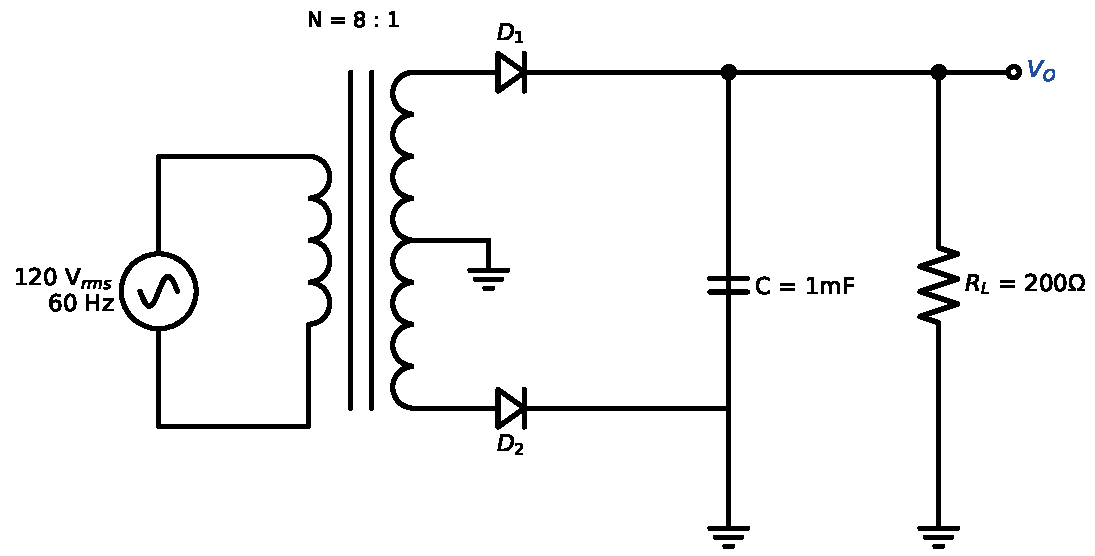
\includegraphics[width=0.9\linewidth,height=5cm,keepaspectratio]{p08_circuit}\end{center}
\solstep{1}{Secondary voltage}The mains peak is $120\sqrt2 = 170$\,V, so the secondary peaks at $\frac{170}{N} = 21.2\,\mathrm{V}$; each half of the center-tapped secondary gets $\hat V_S = 10.6\,\mathrm{V}$.
\solstep{2}{Peak output}At the peak of the input the current flows through one diode (each half of the secondary has its own diode), each dropping $0.7$\,V (tool T1):\[
V_p = \hat V_S - 0.7 = 10.62 - 0.7 = 9.93\,\mathrm{V},\qquad I_L \approx \frac{V_p}{R_L} = 49.6\,\mathrm{m}\mathrm{A}
\]

\solstep{3}{Ripple}Full-wave: the capacitor is recharged every half period, $T = 1/120$\,s. Between recharges the capacitor discharges through $R_L$ (tool T4):\[
V_r \approx V_p\frac{T}{R_LC} = \frac{9.925\times 0.008333}{200\times 0.001} = 414\,\mathrm{m}\mathrm{V}
\]
so the output swings between $V_p = 9.93\,\mathrm{V}$ and $V_p - V_r = 9.51\,\mathrm{V}$ (average $\approx V_p - V_r/2 = 9.72\,\mathrm{V}$).
\solstep{4}{Diode currents}The diodes only conduct during the short recharge interval, so they must deliver a whole period's charge in a short burst (tool T4):\begin{align*}
\sqrt{2V_p/V_r} &= \sqrt{2\times9.925/0.4135} = 6.928 \\
I_{D,av} &= I_L\left(1+\pi\sqrt{2V_p/V_r}\right) = 0.04963\left(1+\pi\times6.928\right) = 1.13\,\mathrm{A} \\
I_{D,max} &= I_L\left(1+2\pi\sqrt{2V_p/V_r}\right) = 2.21\,\mathrm{A}
\end{align*}

\solstep{5}{Peak inverse voltage}When one diode conducts its cathode sits at $V_p = \hat V_S - 0.7$ while its own half of the secondary is at $-\hat V_S$: PIV $= 2\hat V_S - 0.7 = 20.6\,\mathrm{V}$. The diodes must have a reverse breakdown voltage above the PIV.
\solstep{6}{Waveforms}\begin{center}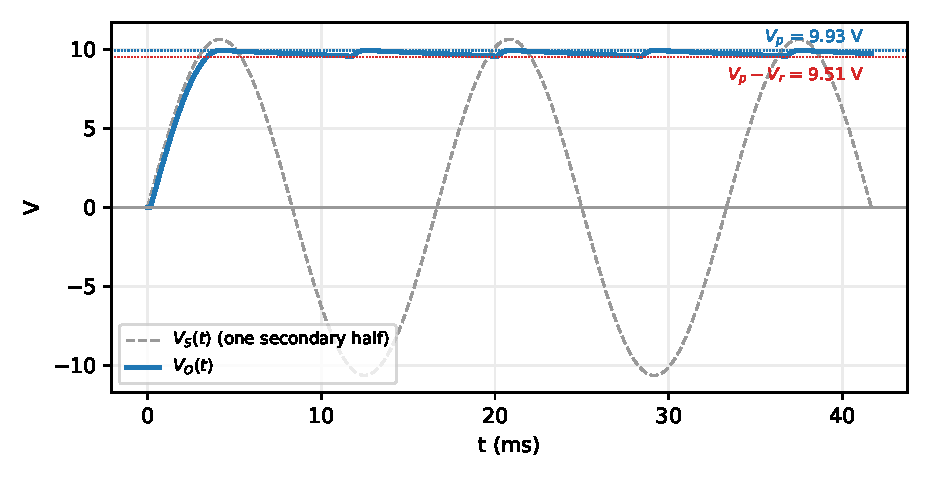
\includegraphics[width=0.7\linewidth,height=5.5cm,keepaspectratio]{p08_wave}\end{center}
 The ripple formula assumes the capacitor discharges for a whole $T$; in reality it is recharged a little earlier, so the true ripple (plotted) is slightly smaller --- the formula errs on the safe side.
\begin{ansbox}
$V_p = 9.93\,\mathrm{V}$,\quad $V_r = 414\,\mathrm{m}\mathrm{V}$,\quad $V_{o,min} = 9.51\,\mathrm{V}$,\quad $I_{D,av} = 1.13\,\mathrm{A}$,\quad $I_{D,max} = 2.21\,\mathrm{A}$,\quad PIV $= 20.6\,\mathrm{V}$
\end{ansbox}

\newpage
\subsection*{Solution 3C.9 \hfill Medium}
\begin{center}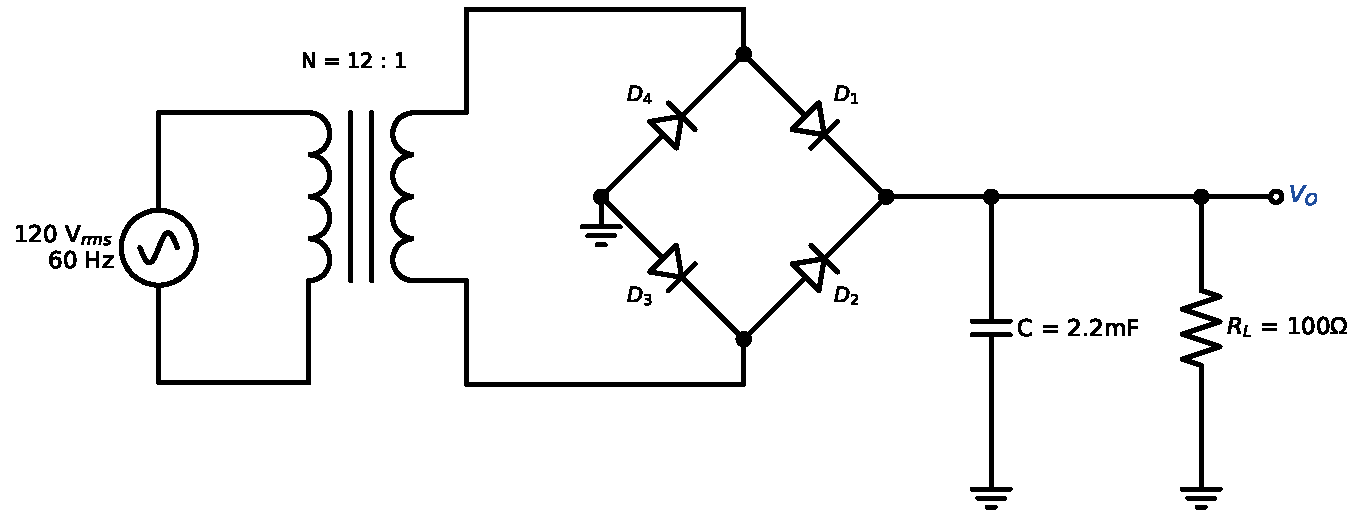
\includegraphics[width=0.9\linewidth,height=5cm,keepaspectratio]{p09_circuit}\end{center}
\solstep{1}{Secondary voltage}The mains peak is $120\sqrt2 = 170$\,V, so the secondary peaks at $\frac{170}{N} = 14.2\,\mathrm{V}$ $=\hat V_S$.
\solstep{2}{Peak output}At the peak of the input the current flows through two diodes in series (one on each side of the bridge), each dropping $0.7$\,V (tool T1):\[
V_p = \hat V_S - 1.4 = 14.17 - 1.4 = 12.8\,\mathrm{V},\qquad I_L \approx \frac{V_p}{R_L} = 128\,\mathrm{m}\mathrm{A}
\]

\solstep{3}{Ripple}Full-wave: the capacitor is recharged every half period, $T = 1/120$\,s. Between recharges the capacitor discharges through $R_L$ (tool T4):\[
V_r \approx V_p\frac{T}{R_LC} = \frac{12.77\times 0.008333}{100\times 0.0022} = 484\,\mathrm{m}\mathrm{V}
\]
so the output swings between $V_p = 12.8\,\mathrm{V}$ and $V_p - V_r = 12.3\,\mathrm{V}$ (average $\approx V_p - V_r/2 = 12.5\,\mathrm{V}$).
\solstep{4}{Diode currents}The diodes only conduct during the short recharge interval, so they must deliver a whole period's charge in a short burst (tool T4):\begin{align*}
\sqrt{2V_p/V_r} &= \sqrt{2\times12.77/0.4836} = 7.266 \\
I_{D,av} &= I_L\left(1+\pi\sqrt{2V_p/V_r}\right) = 0.1277\left(1+\pi\times7.266\right) = 3.04\,\mathrm{A} \\
I_{D,max} &= I_L\left(1+2\pi\sqrt{2V_p/V_r}\right) = 5.96\,\mathrm{A}
\end{align*}

\solstep{5}{Peak inverse voltage}When a pair of diodes conducts, each of the other two sees the output plus one diode drop: PIV $= V_p + 0.7 = \hat V_S - 0.7 = 13.5\,\mathrm{V}$. The diodes must have a reverse breakdown voltage above the PIV.
\solstep{6}{Waveforms}\begin{center}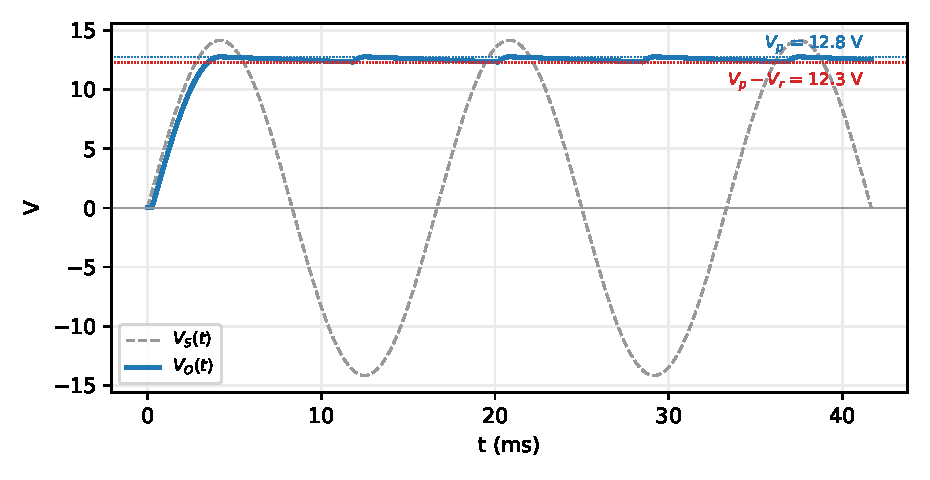
\includegraphics[width=0.7\linewidth,height=5.5cm,keepaspectratio]{p09_wave}\end{center}
 The ripple formula assumes the capacitor discharges for a whole $T$; in reality it is recharged a little earlier, so the true ripple (plotted) is slightly smaller --- the formula errs on the safe side.
\begin{ansbox}
$V_p = 12.8\,\mathrm{V}$,\quad $V_r = 484\,\mathrm{m}\mathrm{V}$,\quad $V_{o,min} = 12.3\,\mathrm{V}$,\quad $I_{D,av} = 3.04\,\mathrm{A}$,\quad $I_{D,max} = 5.96\,\mathrm{A}$,\quad PIV $= 13.5\,\mathrm{V}$
\end{ansbox}

\newpage
\subsection*{Solution 3C.10 \hfill Medium}
\begin{center}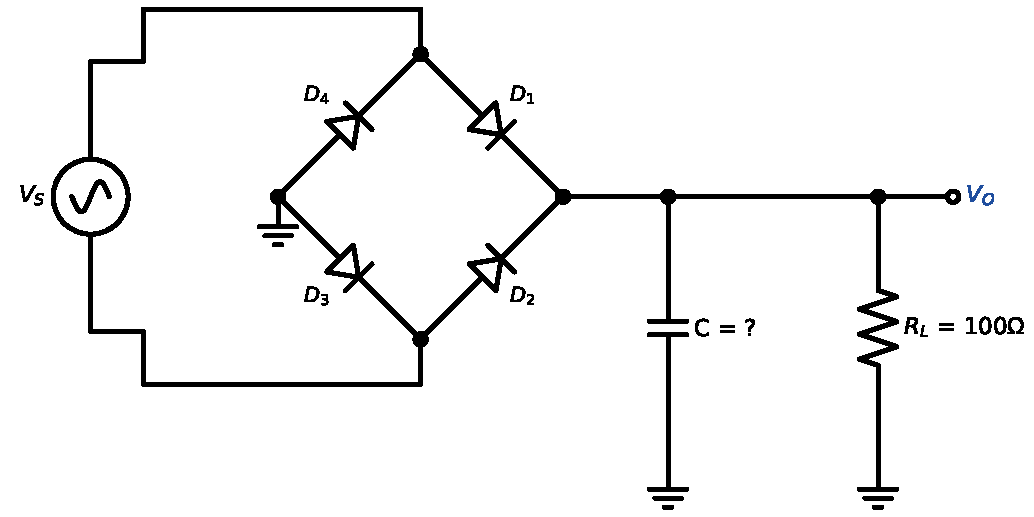
\includegraphics[width=0.9\linewidth,height=5cm,keepaspectratio]{p10_circuit}\end{center}
\solstep{1}{Peak output}At the peak of the input the current flows through two diodes in series (one on each side of the bridge), each dropping $0.7$\,V (tool T1):\[
V_p = \hat V_S - 1.4 = 10 - 1.4 = 8.6\,\mathrm{V},\qquad I_L \approx \frac{V_p}{R_L} = 86\,\mathrm{m}\mathrm{A}
\]

\solstep{2}{Filter capacitor}Full-wave: the capacitor is recharged every half period, $T = 1/120$\,s. Between recharges the capacitor discharges through $R_L$ and loses $V_r \approx V_p\frac{T}{R_LC}$ (tool T4). We need $V_r = 500\,\mathrm{m}\mathrm{V}$:\[
C = \frac{V_pT}{R_LV_r} = \frac{8.6\times 0.008333}{100\times 0.5} = 1.43\,\mathrm{m}\mathrm{F}
\]

\solstep{3}{Diode currents}The diodes only conduct during the short recharge interval, so they must deliver a whole period's charge in a short burst (tool T4):\begin{align*}
\sqrt{2V_p/V_r} &= \sqrt{2\times8.6/0.5} = 5.865 \\
I_{D,av} &= I_L\left(1+\pi\sqrt{2V_p/V_r}\right) = 0.086\left(1+\pi\times5.865\right) = 1.67\,\mathrm{A} \\
I_{D,max} &= I_L\left(1+2\pi\sqrt{2V_p/V_r}\right) = 3.26\,\mathrm{A}
\end{align*}

\solstep{4}{Peak inverse voltage}When a pair of diodes conducts, each of the other two sees the output plus one diode drop: PIV $= V_p + 0.7 = \hat V_S - 0.7 = 9.3\,\mathrm{V}$. The diodes must have a reverse breakdown voltage above the PIV.
\solstep{5}{Waveforms}\begin{center}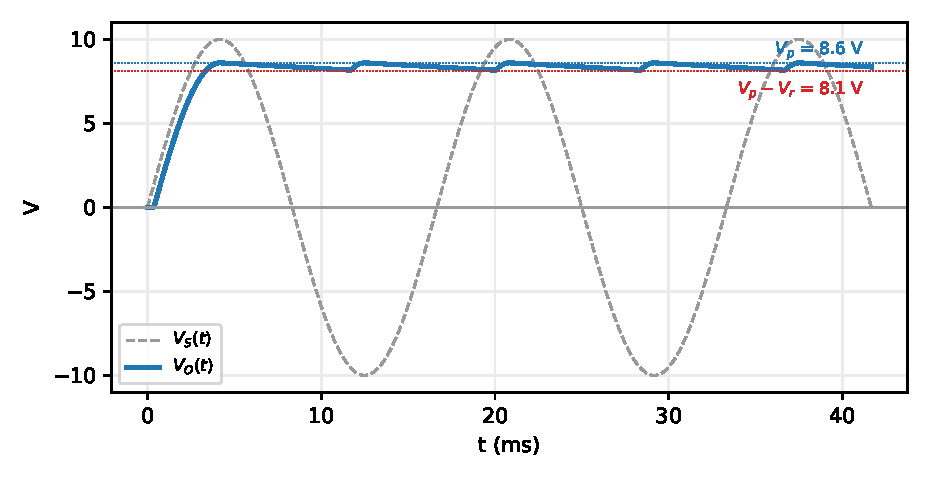
\includegraphics[width=0.7\linewidth,height=5.5cm,keepaspectratio]{p10_wave}\end{center}
 The ripple formula assumes the capacitor discharges for a whole $T$; in reality it is recharged a little earlier, so the true ripple (plotted) is slightly smaller --- the formula errs on the safe side.
\begin{ansbox}
$V_p = 8.6\,\mathrm{V}$,\quad $C = 1.43\,\mathrm{m}\mathrm{F}$,\quad $I_{D,av} = 1.67\,\mathrm{A}$,\quad $I_{D,max} = 3.26\,\mathrm{A}$,\quad PIV $= 9.3\,\mathrm{V}$
\end{ansbox}

\newpage
\subsection*{Solution 3C.11 \hfill Medium}
\begin{center}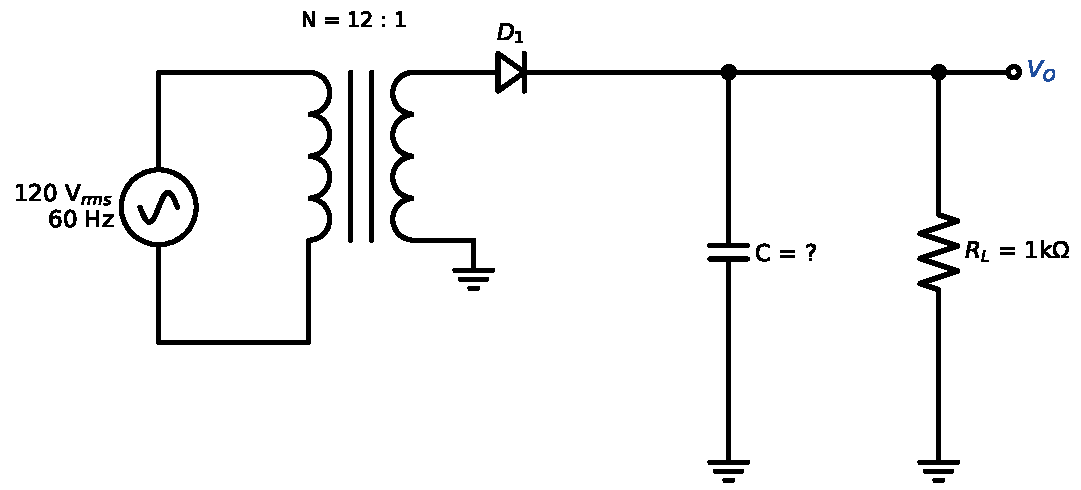
\includegraphics[width=0.9\linewidth,height=5cm,keepaspectratio]{p11_circuit}\end{center}
\solstep{1}{Secondary voltage}The mains peak is $120\sqrt2 = 170$\,V, so the secondary peaks at $\frac{170}{N} = 14.2\,\mathrm{V}$ $=\hat V_S$.
\solstep{2}{Peak output}At the peak of the input the current flows through the single diode, each dropping $0.7$\,V (tool T1):\[
V_p = \hat V_S - 0.7 = 14.17 - 0.7 = 13.5\,\mathrm{V},\qquad I_L \approx \frac{V_p}{R_L} = 13.5\,\mathrm{m}\mathrm{A}
\]

\solstep{3}{Filter capacitor}Half-wave: the capacitor is recharged once per period, $T = 1/60$\,s. Between recharges the capacitor discharges through $R_L$ and loses $V_r \approx V_p\frac{T}{R_LC}$ (tool T4). We need $V_r = V_p - V_{o,min} = 13.47 - 11 = 2.47\,\mathrm{V}$:\[
C = \frac{V_pT}{R_LV_r} = \frac{13.47\times 0.01667}{1000\times 2.467} = 91\,\mu \mathrm{F}
\]

\solstep{4}{Diode currents}The diodes only conduct during the short recharge interval, so they must deliver a whole period's charge in a short burst (tool T4):\begin{align*}
\sqrt{2V_p/V_r} &= \sqrt{2\times13.47/2.467} = 3.304 \\
I_{D,av} &= I_L\left(1+\pi\sqrt{2V_p/V_r}\right) = 0.01347\left(1+\pi\times3.304\right) = 153\,\mathrm{m}\mathrm{A} \\
I_{D,max} &= I_L\left(1+2\pi\sqrt{2V_p/V_r}\right) = 293\,\mathrm{m}\mathrm{A}
\end{align*}

\solstep{5}{Peak inverse voltage}At the negative peak the anode is at $-\hat V_S$ while the capacitor holds the cathode near $V_p$: PIV $= \hat V_S + V_p = 2\hat V_S - 0.7 = 27.6\,\mathrm{V}$. The diodes must have a reverse breakdown voltage above the PIV.
\solstep{6}{Waveforms}\begin{center}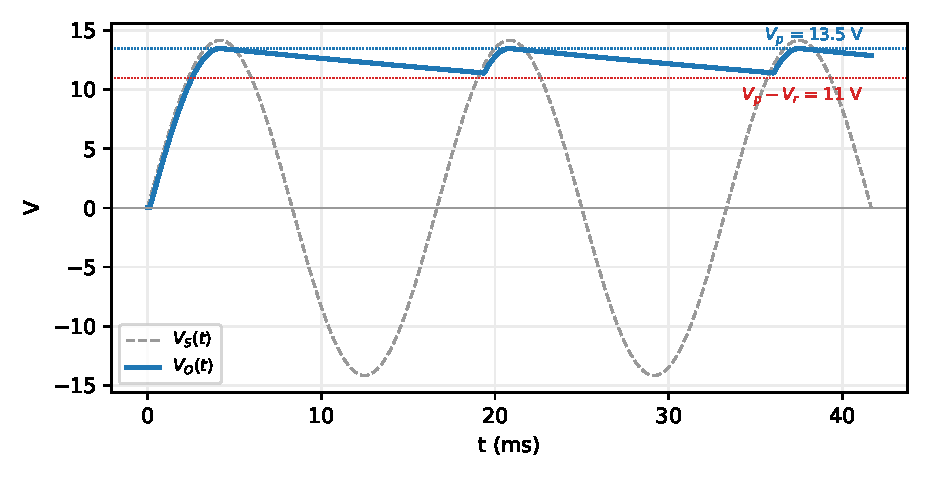
\includegraphics[width=0.7\linewidth,height=5.5cm,keepaspectratio]{p11_wave}\end{center}
 The ripple formula assumes the capacitor discharges for a whole $T$; in reality it is recharged a little earlier, so the true ripple (plotted) is slightly smaller --- the formula errs on the safe side.
\begin{ansbox}
$V_p = 13.5\,\mathrm{V}$,\quad $C = 91\,\mu \mathrm{F}$,\quad $I_{D,av} = 153\,\mathrm{m}\mathrm{A}$,\quad $I_{D,max} = 293\,\mathrm{m}\mathrm{A}$,\quad PIV $= 27.6\,\mathrm{V}$
\end{ansbox}

\newpage
\subsection*{Solution 3C.12 \hfill Medium}
\begin{center}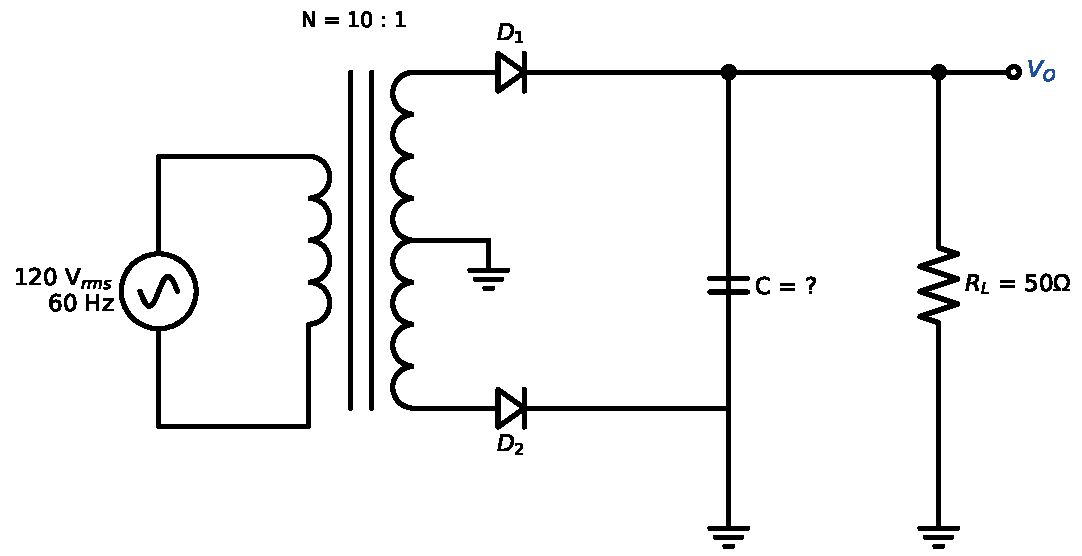
\includegraphics[width=0.9\linewidth,height=5cm,keepaspectratio]{p12_circuit}\end{center}
\solstep{1}{Secondary voltage}The mains peak is $120\sqrt2 = 170$\,V, so the secondary peaks at $\frac{170}{N} = 17\,\mathrm{V}$; each half of the center-tapped secondary gets $\hat V_S = 8.5\,\mathrm{V}$.
\solstep{2}{Peak output}At the peak of the input the current flows through one diode (each half of the secondary has its own diode), each dropping $0.7$\,V (tool T1):\[
V_p = \hat V_S - 0.7 = 8.5 - 0.7 = 7.8\,\mathrm{V},\qquad I_L \approx \frac{V_p}{R_L} = 156\,\mathrm{m}\mathrm{A}
\]

\solstep{3}{Filter capacitor}Full-wave: the capacitor is recharged every half period, $T = 1/120$\,s. Between recharges the capacitor discharges through $R_L$ and loses $V_r \approx V_p\frac{T}{R_LC}$ (tool T4). We need $V_r = 400\,\mathrm{m}\mathrm{V}$:\[
C = \frac{V_pT}{R_LV_r} = \frac{7.8\times 0.008333}{50\times 0.4} = 3.25\,\mathrm{m}\mathrm{F}
\]

\solstep{4}{Diode currents}The diodes only conduct during the short recharge interval, so they must deliver a whole period's charge in a short burst (tool T4):\begin{align*}
\sqrt{2V_p/V_r} &= \sqrt{2\times7.8/0.4} = 6.245 \\
I_{D,av} &= I_L\left(1+\pi\sqrt{2V_p/V_r}\right) = 0.156\left(1+\pi\times6.245\right) = 3.22\,\mathrm{A} \\
I_{D,max} &= I_L\left(1+2\pi\sqrt{2V_p/V_r}\right) = 6.28\,\mathrm{A}
\end{align*}

\solstep{5}{Peak inverse voltage}When one diode conducts its cathode sits at $V_p = \hat V_S - 0.7$ while its own half of the secondary is at $-\hat V_S$: PIV $= 2\hat V_S - 0.7 = 16.3\,\mathrm{V}$. The diodes must have a reverse breakdown voltage above the PIV.
\solstep{6}{Waveforms}\begin{center}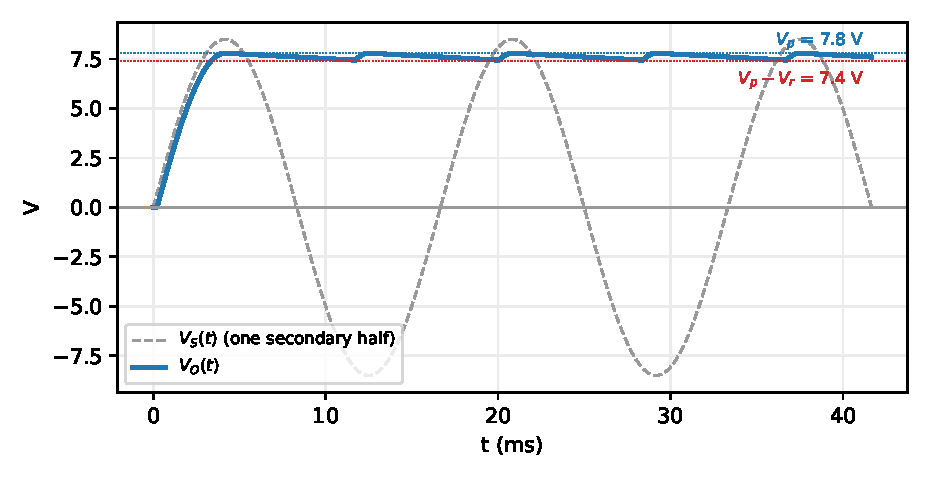
\includegraphics[width=0.7\linewidth,height=5.5cm,keepaspectratio]{p12_wave}\end{center}
 The ripple formula assumes the capacitor discharges for a whole $T$; in reality it is recharged a little earlier, so the true ripple (plotted) is slightly smaller --- the formula errs on the safe side.
\begin{ansbox}
$V_p = 7.8\,\mathrm{V}$,\quad $C = 3.25\,\mathrm{m}\mathrm{F}$,\quad $I_{D,av} = 3.22\,\mathrm{A}$,\quad $I_{D,max} = 6.28\,\mathrm{A}$,\quad PIV $= 16.3\,\mathrm{V}$
\end{ansbox}

\newpage
\subsection*{Solution 3C.13 \hfill Hard}
\begin{center}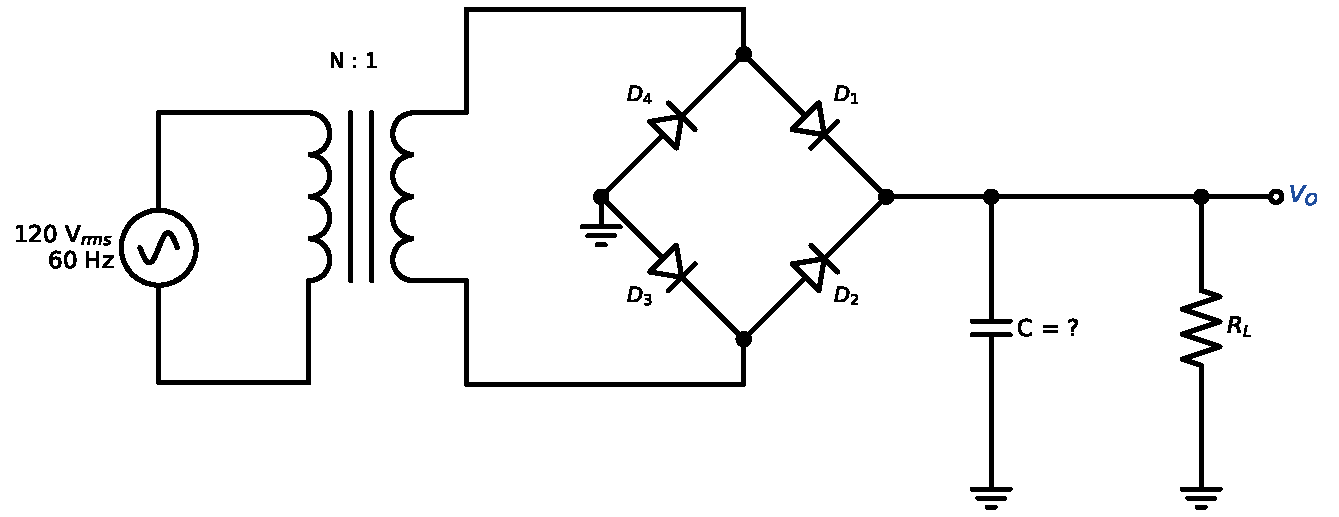
\includegraphics[width=0.9\linewidth,height=5cm,keepaspectratio]{p13_circuit}\end{center}
\solstep{1}{Worst-case load}The ripple is largest at the largest current, so design for $I_L = 400\,\mathrm{m}\mathrm{A}$: the load looks like $R_L = \frac{V_o}{I_{L,max}} = \frac{3}{0.4} = 7.5\,\Omega$.
\solstep{2}{Transformer ratio}The mains peak is $120\sqrt2 = 170$\,V. The current passes through two diodes in series (one on each side of the bridge), so the secondary must peak at $\hat V_S = V_o + 1.4 = 4.4\,\mathrm{V}$, and $N = \frac{170}{\hat V_S} = \frac{170}{4.4} = 38.64$.
\solstep{3}{Filter capacitor}Full-wave: the capacitor is recharged every half period, $T=1/120$\,s. Ripple $V_r = V_p\frac{T}{R_LC}$ and $K_r = \frac{V_r}{V_p} = \frac{T}{R_LC}$ (tool T4), so\[
C = \frac{T}{R_L K_r} = \frac{0.008333}{7.5\times 0.05} = 22.2\,\mathrm{m}\mathrm{F}
\]

\solstep{4}{Diode currents}The diodes only conduct during the short recharge interval, so they must deliver a whole period's charge in a short burst (tool T4):\begin{align*}
\sqrt{2V_p/V_r} &= \sqrt{2\times3/0.15} = 6.325 \\
I_{D,av} &= I_L\left(1+\pi\sqrt{2V_p/V_r}\right) = 0.4\left(1+\pi\times6.325\right) = 8.35\,\mathrm{A} \\
I_{D,max} &= I_L\left(1+2\pi\sqrt{2V_p/V_r}\right) = 16.3\,\mathrm{A}
\end{align*}

\solstep{5}{Peak inverse voltage}When a pair of diodes conducts, each of the other two sees the output plus one diode drop: PIV $= V_p + 0.7 = \hat V_S - 0.7 = 3.7\,\mathrm{V}$. The diodes must have a reverse breakdown voltage above the PIV.
\solstep{6}{Waveforms}\begin{center}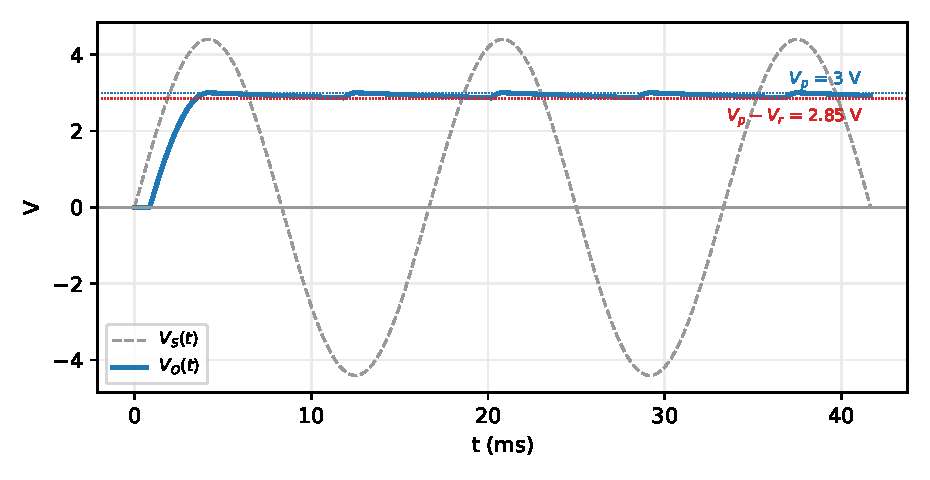
\includegraphics[width=0.7\linewidth,height=5.5cm,keepaspectratio]{p13_wave}\end{center}
 The ripple formula assumes the capacitor discharges for a whole $T$; in reality it is recharged a little earlier, so the true ripple (plotted) is slightly smaller --- the formula errs on the safe side.
\begin{ansbox}
$N = 38.64$,\quad $C = 22.2\,\mathrm{m}\mathrm{F}$,\quad $R_L = 7.5\,\Omega$,\quad $I_{D,av} = 8.35\,\mathrm{A}$,\quad $I_{D,max} = 16.3\,\mathrm{A}$,\quad PIV $= 3.7\,\mathrm{V}$
\end{ansbox}

\newpage
\subsection*{Solution 3C.14 \hfill Hard}
\begin{center}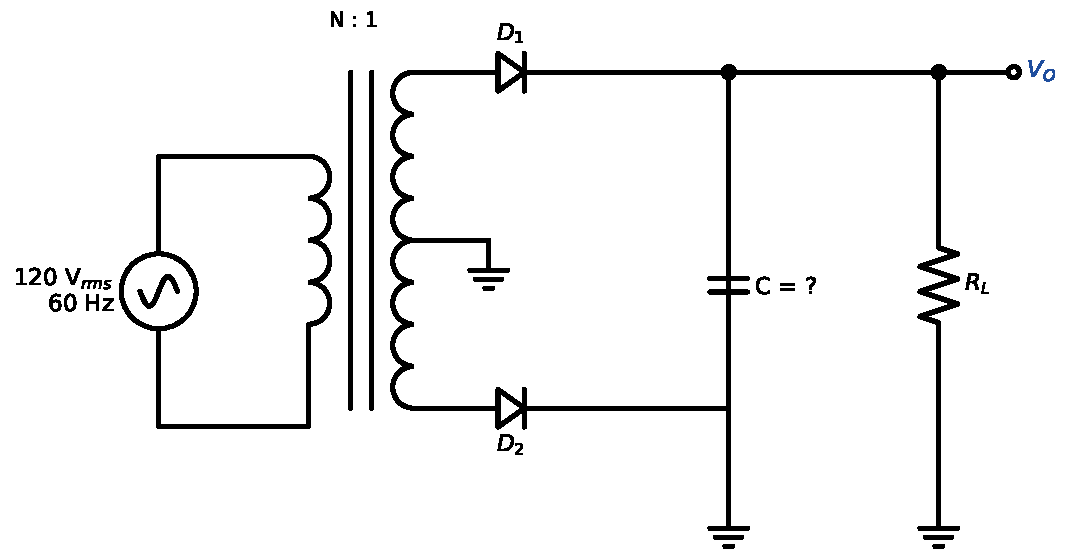
\includegraphics[width=0.9\linewidth,height=5cm,keepaspectratio]{p14_circuit}\end{center}
\solstep{1}{Worst-case load}The ripple is largest at the largest current, so design for $I_L = 1.5\,\mathrm{A}$: the load looks like $R_L = \frac{V_o}{I_{L,max}} = \frac{5}{1.5} = 3.33\,\Omega$.
\solstep{2}{Transformer ratio}The mains peak is $120\sqrt2 = 170$\,V. Each half of the secondary must peak at $\hat V_S = V_o + 0.7 = 5.7\,\mathrm{V}$, so the whole secondary peaks at $2\hat V_S = 11.4\,\mathrm{V}$ and $N = \frac{170}{2(V_o+0.7)} = \frac{170}{11.4} = 14.91$.
\solstep{3}{Filter capacitor}Full-wave: the capacitor is recharged every half period, $T=1/120$\,s. Ripple $V_r = V_p\frac{T}{R_LC}$ and $K_r = \frac{V_r}{V_p} = \frac{T}{R_LC}$ (tool T4), so\[
C = \frac{T}{R_L K_r} = \frac{0.008333}{3.333\times 0.1} = 25\,\mathrm{m}\mathrm{F}
\]

\solstep{4}{Diode currents}The diodes only conduct during the short recharge interval, so they must deliver a whole period's charge in a short burst (tool T4):\begin{align*}
\sqrt{2V_p/V_r} &= \sqrt{2\times5/0.5} = 4.472 \\
I_{D,av} &= I_L\left(1+\pi\sqrt{2V_p/V_r}\right) = 1.5\left(1+\pi\times4.472\right) = 22.6\,\mathrm{A} \\
I_{D,max} &= I_L\left(1+2\pi\sqrt{2V_p/V_r}\right) = 43.6\,\mathrm{A}
\end{align*}

\solstep{5}{Peak inverse voltage}When one diode conducts its cathode sits at $V_p = \hat V_S - 0.7$ while its own half of the secondary is at $-\hat V_S$: PIV $= 2\hat V_S - 0.7 = 10.7\,\mathrm{V}$. The diodes must have a reverse breakdown voltage above the PIV.
\solstep{6}{Waveforms}\begin{center}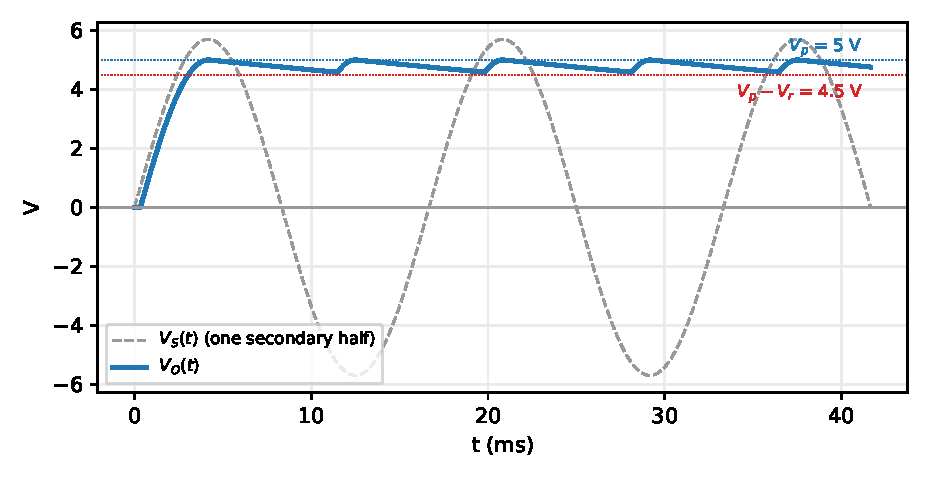
\includegraphics[width=0.7\linewidth,height=5.5cm,keepaspectratio]{p14_wave}\end{center}
 The ripple formula assumes the capacitor discharges for a whole $T$; in reality it is recharged a little earlier, so the true ripple (plotted) is slightly smaller --- the formula errs on the safe side.
\begin{ansbox}
$N = 14.91$,\quad $C = 25\,\mathrm{m}\mathrm{F}$,\quad $R_L = 3.33\,\Omega$,\quad $I_{D,av} = 22.6\,\mathrm{A}$,\quad $I_{D,max} = 43.6\,\mathrm{A}$,\quad PIV $= 10.7\,\mathrm{V}$
\end{ansbox}

\newpage
\subsection*{Solution 3C.15 \hfill Hard}
\begin{center}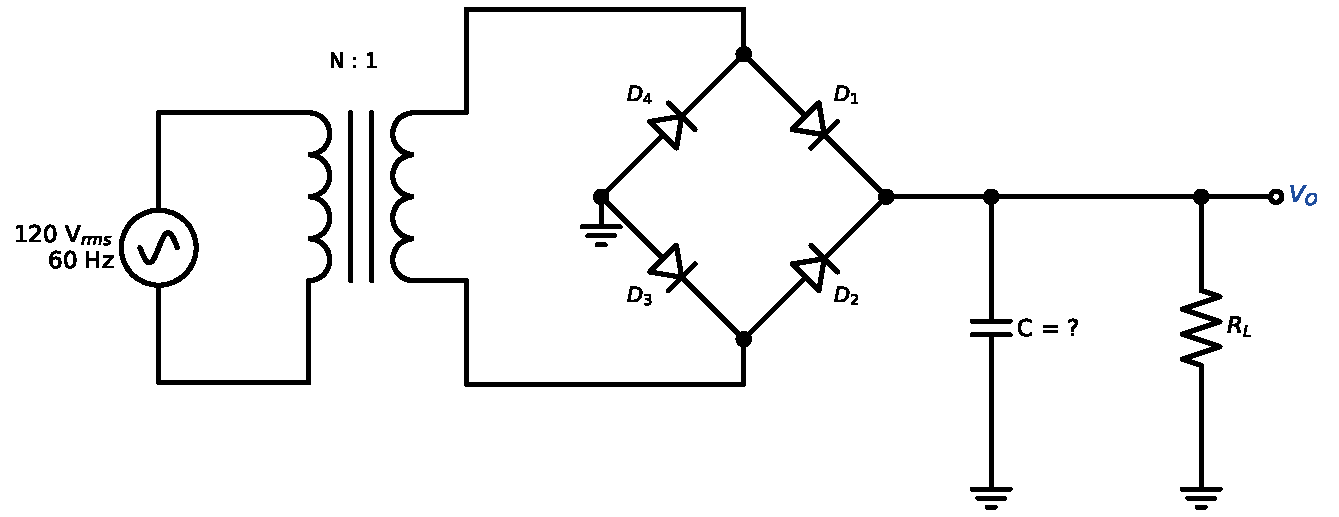
\includegraphics[width=0.9\linewidth,height=5cm,keepaspectratio]{p15_circuit}\end{center}
\solstep{1}{Worst-case load}The ripple is largest at the largest current, so design for $I_L = 1\,\mathrm{A}$: the load looks like $R_L = \frac{V_o}{I_{L,max}} = \frac{12}{1} = 12\,\Omega$.
\solstep{2}{Transformer ratio}The mains peak is $120\sqrt2 = 170$\,V. The current passes through two diodes in series (one on each side of the bridge), so the secondary must peak at $\hat V_S = V_o + 1.4 = 13.4\,\mathrm{V}$, and $N = \frac{170}{\hat V_S} = \frac{170}{13.4} = 12.69$.
\solstep{3}{Filter capacitor}Full-wave: the capacitor is recharged every half period, $T=1/120$\,s. Ripple $V_r = V_p\frac{T}{R_LC}$ and $K_r = \frac{V_r}{V_p} = \frac{T}{R_LC}$ (tool T4), so\[
C = \frac{T}{R_L K_r} = \frac{0.008333}{12\times 0.05} = 13.9\,\mathrm{m}\mathrm{F}
\]

\solstep{4}{Diode currents}The diodes only conduct during the short recharge interval, so they must deliver a whole period's charge in a short burst (tool T4):\begin{align*}
\sqrt{2V_p/V_r} &= \sqrt{2\times12/0.6} = 6.325 \\
I_{D,av} &= I_L\left(1+\pi\sqrt{2V_p/V_r}\right) = 1\left(1+\pi\times6.325\right) = 20.9\,\mathrm{A} \\
I_{D,max} &= I_L\left(1+2\pi\sqrt{2V_p/V_r}\right) = 40.7\,\mathrm{A}
\end{align*}

\solstep{5}{Peak inverse voltage}When a pair of diodes conducts, each of the other two sees the output plus one diode drop: PIV $= V_p + 0.7 = \hat V_S - 0.7 = 12.7\,\mathrm{V}$. The diodes must have a reverse breakdown voltage above the PIV.
\solstep{6}{Waveforms}\begin{center}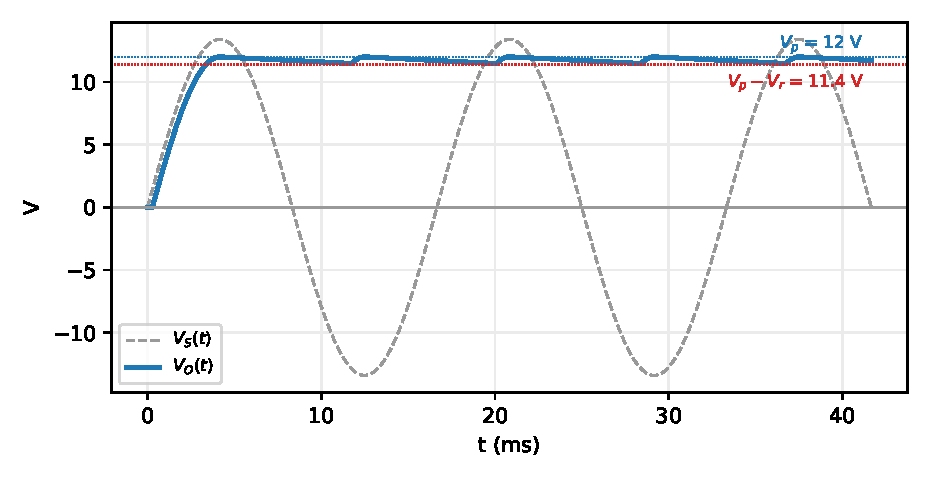
\includegraphics[width=0.7\linewidth,height=5.5cm,keepaspectratio]{p15_wave}\end{center}
 The ripple formula assumes the capacitor discharges for a whole $T$; in reality it is recharged a little earlier, so the true ripple (plotted) is slightly smaller --- the formula errs on the safe side.
\begin{ansbox}
$N = 12.69$,\quad $C = 13.9\,\mathrm{m}\mathrm{F}$,\quad $R_L = 12\,\Omega$,\quad $I_{D,av} = 20.9\,\mathrm{A}$,\quad $I_{D,max} = 40.7\,\mathrm{A}$,\quad PIV $= 12.7\,\mathrm{V}$
\end{ansbox}

\newpage
\subsection*{Solution 3C.16 \hfill Hard}
\begin{center}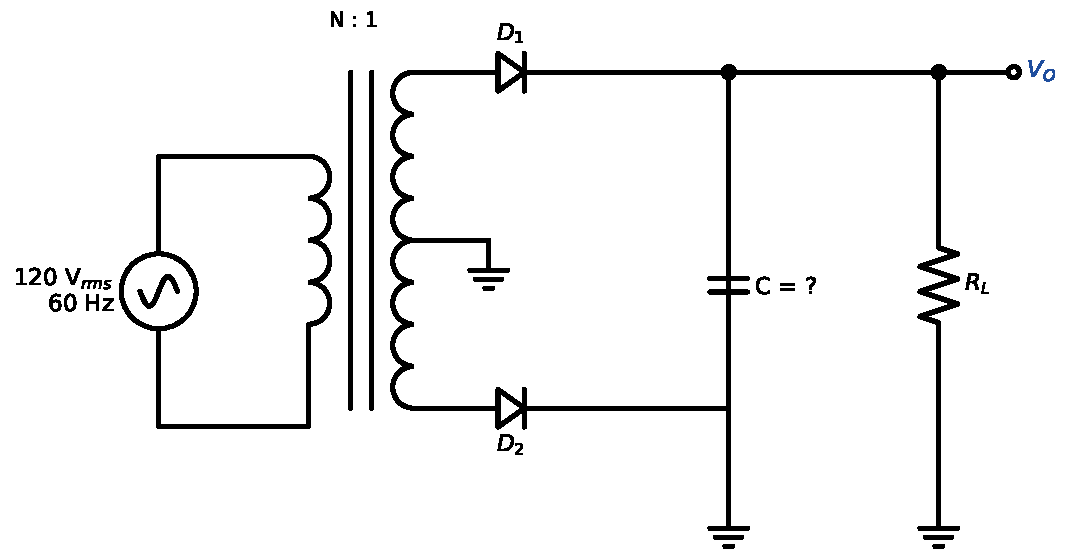
\includegraphics[width=0.9\linewidth,height=5cm,keepaspectratio]{p16_circuit}\end{center}
\solstep{1}{Worst-case load}The ripple is largest at the largest current, so design for $I_L = 500\,\mathrm{m}\mathrm{A}$: the load looks like $R_L = \frac{V_o}{I_{L,max}} = \frac{9}{0.5} = 18\,\Omega$.
\solstep{2}{Transformer ratio}The mains peak is $120\sqrt2 = 170$\,V. Each half of the secondary must peak at $\hat V_S = V_o + 0.7 = 9.7\,\mathrm{V}$, so the whole secondary peaks at $2\hat V_S = 19.4\,\mathrm{V}$ and $N = \frac{170}{2(V_o+0.7)} = \frac{170}{19.4} = 8.763$.
\solstep{3}{Filter capacitor}Full-wave: the capacitor is recharged every half period, $T=1/120$\,s. Ripple $V_r = V_p\frac{T}{R_LC}$ and $K_r = \frac{V_r}{V_p} = \frac{T}{R_LC}$ (tool T4), so\[
C = \frac{T}{R_L K_r} = \frac{0.008333}{18\times 0.05} = 9.26\,\mathrm{m}\mathrm{F}
\]

\solstep{4}{Diode currents}The diodes only conduct during the short recharge interval, so they must deliver a whole period's charge in a short burst (tool T4):\begin{align*}
\sqrt{2V_p/V_r} &= \sqrt{2\times9/0.45} = 6.325 \\
I_{D,av} &= I_L\left(1+\pi\sqrt{2V_p/V_r}\right) = 0.5\left(1+\pi\times6.325\right) = 10.4\,\mathrm{A} \\
I_{D,max} &= I_L\left(1+2\pi\sqrt{2V_p/V_r}\right) = 20.4\,\mathrm{A}
\end{align*}

\solstep{5}{Peak inverse voltage}When one diode conducts its cathode sits at $V_p = \hat V_S - 0.7$ while its own half of the secondary is at $-\hat V_S$: PIV $= 2\hat V_S - 0.7 = 18.7\,\mathrm{V}$. The diodes must have a reverse breakdown voltage above the PIV.
\solstep{6}{Waveforms}\begin{center}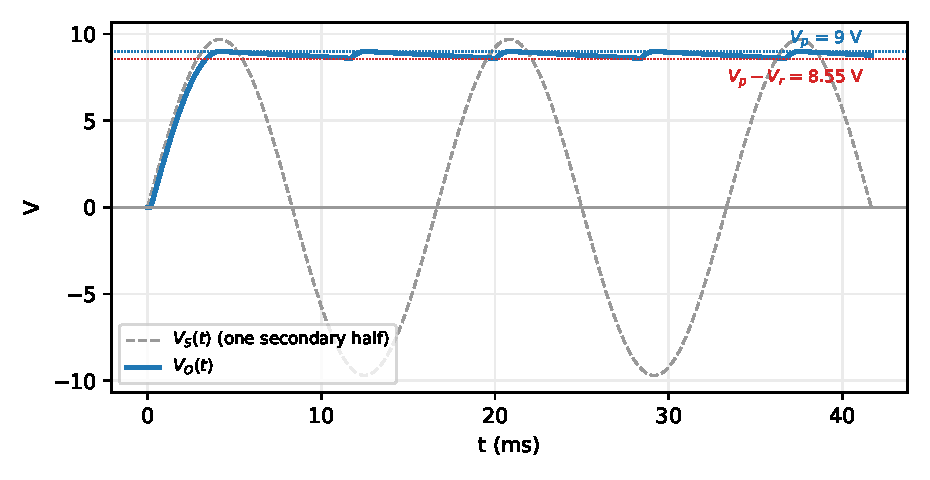
\includegraphics[width=0.7\linewidth,height=5.5cm,keepaspectratio]{p16_wave}\end{center}
 The ripple formula assumes the capacitor discharges for a whole $T$; in reality it is recharged a little earlier, so the true ripple (plotted) is slightly smaller --- the formula errs on the safe side.
\begin{ansbox}
$N = 8.763$,\quad $C = 9.26\,\mathrm{m}\mathrm{F}$,\quad $R_L = 18\,\Omega$,\quad $I_{D,av} = 10.4\,\mathrm{A}$,\quad $I_{D,max} = 20.4\,\mathrm{A}$,\quad PIV $= 18.7\,\mathrm{V}$
\end{ansbox}

\newpage
\subsection*{Solution 3C.17 \hfill Hard}
\begin{center}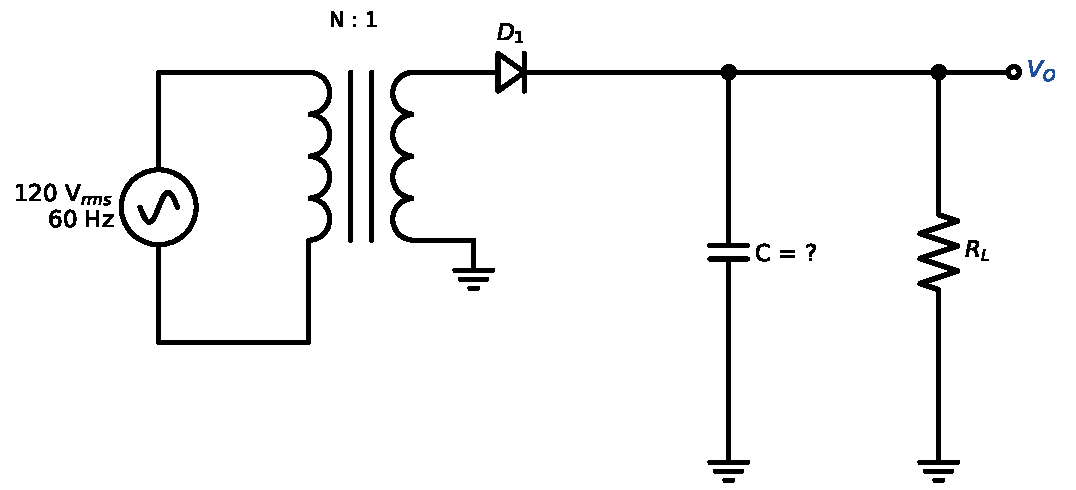
\includegraphics[width=0.9\linewidth,height=5cm,keepaspectratio]{p17_circuit}\end{center}
\solstep{1}{Worst-case load}The ripple is largest at the largest current, so design for $I_L = 100\,\mathrm{m}\mathrm{A}$: the load looks like $R_L = \frac{V_o}{I_{L,max}} = \frac{5}{0.1} = 50\,\Omega$.
\solstep{2}{Transformer ratio}The mains peak is $120\sqrt2 = 170$\,V. The current passes through the single diode, so the secondary must peak at $\hat V_S = V_o + 0.7 = 5.7\,\mathrm{V}$, and $N = \frac{170}{\hat V_S} = \frac{170}{5.7} = 29.82$.
\solstep{3}{Filter capacitor}Half-wave: the capacitor is recharged once per period, $T=1/60$\,s. Ripple $V_r = V_p\frac{T}{R_LC}$ and $K_r = \frac{V_r}{V_p} = \frac{T}{R_LC}$ (tool T4), so\[
C = \frac{T}{R_L K_r} = \frac{0.01667}{50\times 0.1} = 3.33\,\mathrm{m}\mathrm{F}
\]

\solstep{4}{Diode currents}The diodes only conduct during the short recharge interval, so they must deliver a whole period's charge in a short burst (tool T4):\begin{align*}
\sqrt{2V_p/V_r} &= \sqrt{2\times5/0.5} = 4.472 \\
I_{D,av} &= I_L\left(1+\pi\sqrt{2V_p/V_r}\right) = 0.1\left(1+\pi\times4.472\right) = 1.5\,\mathrm{A} \\
I_{D,max} &= I_L\left(1+2\pi\sqrt{2V_p/V_r}\right) = 2.91\,\mathrm{A}
\end{align*}

\solstep{5}{Peak inverse voltage}At the negative peak the anode is at $-\hat V_S$ while the capacitor holds the cathode near $V_p$: PIV $= \hat V_S + V_p = 2\hat V_S - 0.7 = 10.7\,\mathrm{V}$. The diodes must have a reverse breakdown voltage above the PIV.
\solstep{6}{Waveforms}\begin{center}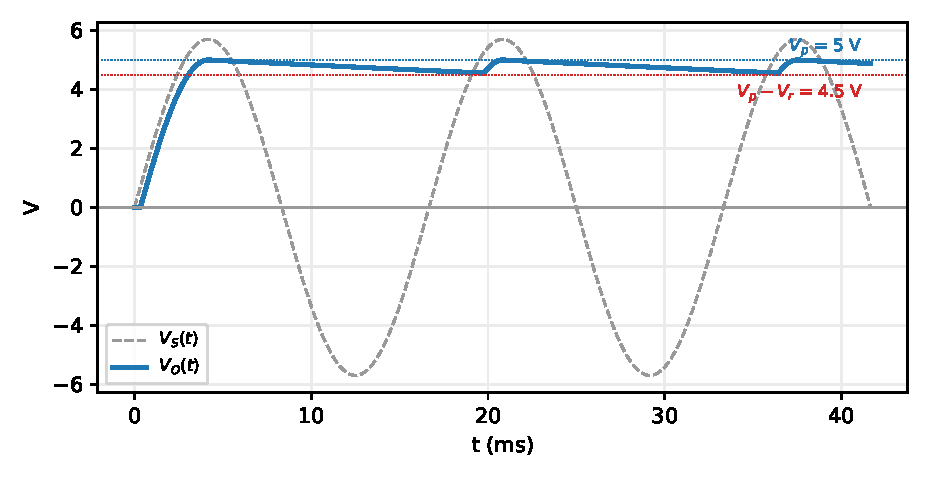
\includegraphics[width=0.7\linewidth,height=5.5cm,keepaspectratio]{p17_wave}\end{center}
 The ripple formula assumes the capacitor discharges for a whole $T$; in reality it is recharged a little earlier, so the true ripple (plotted) is slightly smaller --- the formula errs on the safe side.
\begin{ansbox}
$N = 29.82$,\quad $C = 3.33\,\mathrm{m}\mathrm{F}$,\quad $R_L = 50\,\Omega$,\quad $I_{D,av} = 1.5\,\mathrm{A}$,\quad $I_{D,max} = 2.91\,\mathrm{A}$,\quad PIV $= 10.7\,\mathrm{V}$
\end{ansbox}

\newpage
\subsection*{Solution 3C.18 \hfill Hard}
\begin{center}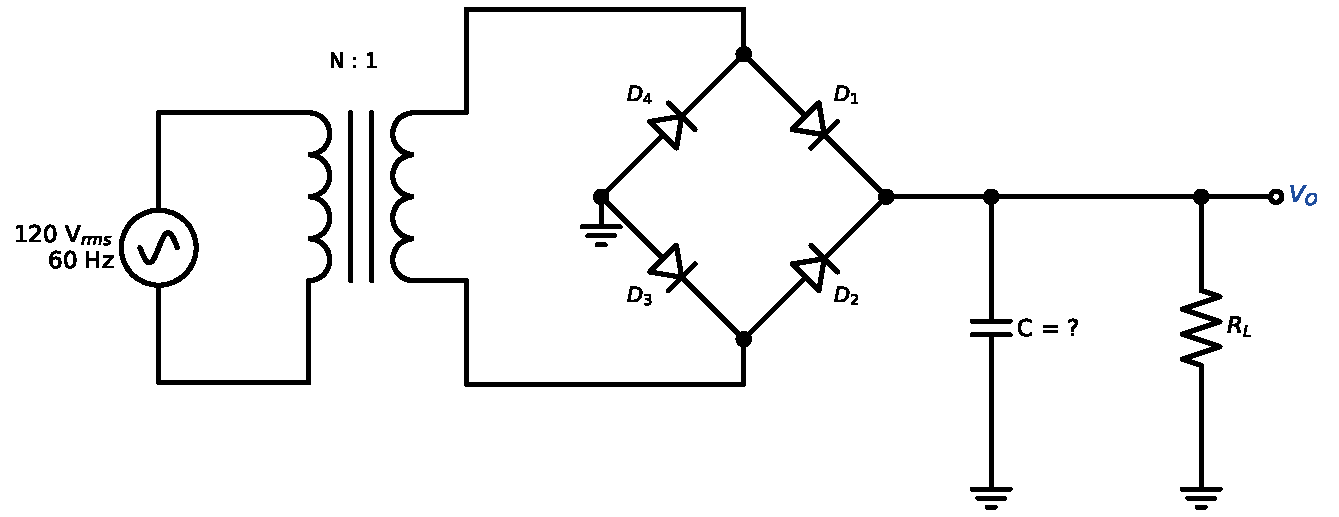
\includegraphics[width=0.9\linewidth,height=5cm,keepaspectratio]{p18_circuit}\end{center}
\solstep{1}{Worst-case load}The ripple is largest at the largest current, so design for $I_L = 800\,\mathrm{m}\mathrm{A}$: the load looks like $R_L = \frac{V_o}{I_{L,max}} = \frac{15}{0.8} = 18.8\,\Omega$.
\solstep{2}{Transformer ratio}The mains peak is $120\sqrt2 = 170$\,V. The current passes through two diodes in series (one on each side of the bridge), so the secondary must peak at $\hat V_S = V_o + 1.4 = 16.4\,\mathrm{V}$, and $N = \frac{170}{\hat V_S} = \frac{170}{16.4} = 10.37$.
\solstep{3}{Filter capacitor}Full-wave: the capacitor is recharged every half period, $T=1/120$\,s. Ripple $V_r = V_p\frac{T}{R_LC}$ and $K_r = \frac{V_r}{V_p} = \frac{T}{R_LC}$ (tool T4), so\[
C = \frac{T}{R_L K_r} = \frac{0.008333}{18.75\times 0.05} = 8.89\,\mathrm{m}\mathrm{F}
\]

\solstep{4}{Diode currents}The diodes only conduct during the short recharge interval, so they must deliver a whole period's charge in a short burst (tool T4):\begin{align*}
\sqrt{2V_p/V_r} &= \sqrt{2\times15/0.75} = 6.325 \\
I_{D,av} &= I_L\left(1+\pi\sqrt{2V_p/V_r}\right) = 0.8\left(1+\pi\times6.325\right) = 16.7\,\mathrm{A} \\
I_{D,max} &= I_L\left(1+2\pi\sqrt{2V_p/V_r}\right) = 32.6\,\mathrm{A}
\end{align*}

\solstep{5}{Peak inverse voltage}When a pair of diodes conducts, each of the other two sees the output plus one diode drop: PIV $= V_p + 0.7 = \hat V_S - 0.7 = 15.7\,\mathrm{V}$. The diodes must have a reverse breakdown voltage above the PIV.
\solstep{6}{Waveforms}\begin{center}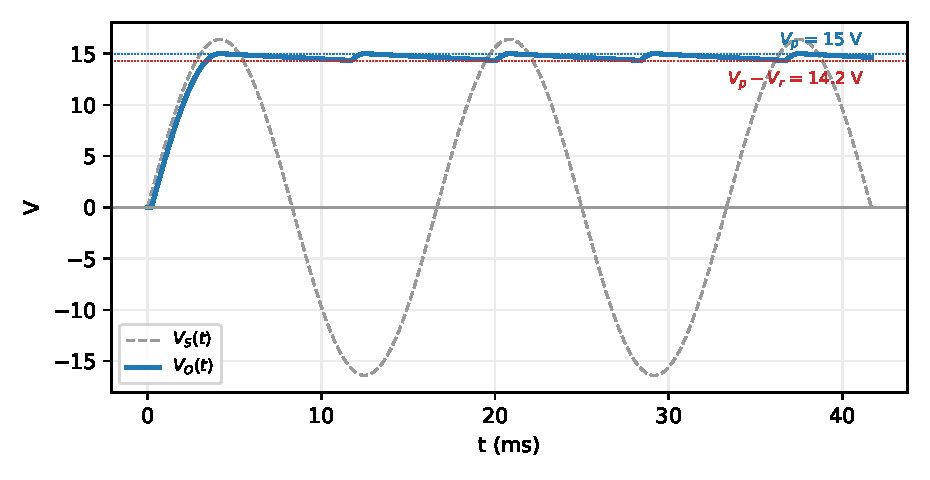
\includegraphics[width=0.7\linewidth,height=5.5cm,keepaspectratio]{p18_wave}\end{center}
 The ripple formula assumes the capacitor discharges for a whole $T$; in reality it is recharged a little earlier, so the true ripple (plotted) is slightly smaller --- the formula errs on the safe side.
\begin{ansbox}
$N = 10.37$,\quad $C = 8.89\,\mathrm{m}\mathrm{F}$,\quad $R_L = 18.8\,\Omega$,\quad $I_{D,av} = 16.7\,\mathrm{A}$,\quad $I_{D,max} = 32.6\,\mathrm{A}$,\quad PIV $= 15.7\,\mathrm{V}$
\end{ansbox}

\end{document}
